% Capitolul 2: Distribuții Statistice pentru Piețele Financiare
% Statistica Piețelor Financiare
% Program de licență, Academia de Studii Economice din București

\documentclass[9pt, aspectratio=169, t]{beamer}

% Asigură încadrarea conținutului pe diapozitive
\setbeamersize{text margin left=8mm, text margin right=8mm}

%=============================================================================
% CONFIGURARE TEMĂ ȘI STIL
%=============================================================================
\usetheme{default}
% Utilizăm tema implicită pentru control curat al antetului/subsolului

% Paletă de Culori (potrivită cu PDF-ul Redispatch)
\definecolor{MainBlue}{RGB}{26, 58, 110}
\definecolor{AccentBlue}{RGB}{26, 58, 110}
\definecolor{IDAred}{RGB}{205, 0, 0}
\definecolor{DarkGray}{RGB}{51, 51, 51}
\definecolor{MediumGray}{RGB}{128, 128, 128}
\definecolor{LightGray}{RGB}{248, 248, 248}
\definecolor{VeryLightGray}{RGB}{235, 235, 235}
\definecolor{KeynoteGray}{RGB}{218, 218, 218}
\definecolor{SectionGray}{RGB}{120, 120, 120}
\definecolor{FooterGray}{RGB}{100, 100, 100}
\definecolor{Crimson}{RGB}{220, 53, 69}
\definecolor{Forest}{RGB}{46, 125, 50}
\definecolor{Amber}{RGB}{181, 133, 63}
\definecolor{Orange}{RGB}{230, 126, 34}
\definecolor{Purple}{RGB}{142, 68, 173}

% Fundal gradient (gradient Keynote exact 315°: alb la RGB 218,218,218)
\setbeamertemplate{background}{%
    \begin{tikzpicture}[remember picture, overlay]
        \shade[shading=axis, shading angle=315,
        top color=white, bottom color=KeynoteGray]
        (current page.south west) rectangle (current page.north east);
    \end{tikzpicture}%
}
% Culoare solidă de rezervă pentru compatibilitate
\setbeamercolor{background canvas}{bg=}

\setbeamercolor{palette primary}{bg=MainBlue, fg=white}
\setbeamercolor{palette secondary}{bg=MainBlue!85, fg=white}
\setbeamercolor{palette tertiary}{bg=MainBlue!70, fg=white}
\setbeamercolor{structure}{fg=MainBlue}
\setbeamercolor{title}{fg=IDAred}
\setbeamercolor{frametitle}{fg=IDAred, bg=}
\setbeamercolor{block title}{bg=MainBlue, fg=white}
\setbeamercolor{block body}{bg=VeryLightGray, fg=DarkGray}
\setbeamercolor{block title alerted}{bg=Crimson, fg=white}
\setbeamercolor{block body alerted}{bg=Crimson!8, fg=DarkGray}
\setbeamercolor{block title example}{bg=Forest, fg=white}
\setbeamercolor{block body example}{bg=Forest!8, fg=DarkGray}
\setbeamercolor{item}{fg=MainBlue}

% Culori subsol (suprascriu albastrul temei Madrid)
\setbeamercolor{author in head/foot}{fg=FooterGray, bg=}
\setbeamercolor{title in head/foot}{fg=FooterGray, bg=}
\setbeamercolor{date in head/foot}{fg=FooterGray, bg=}
\setbeamercolor{section in head/foot}{fg=FooterGray, bg=}
\setbeamercolor{subsection in head/foot}{fg=FooterGray, bg=}

% Stiluri marcatori (se aplică peste tot inclusiv în blocuri)
\setbeamertemplate{itemize item}{\color{MainBlue}$\boxdot$}
\setbeamertemplate{itemize subitem}{\color{MainBlue}$\blacktriangleright$}
\setbeamertemplate{itemize subsubitem}{\color{MainBlue}\tiny$\bullet$}
\setbeamertemplate{itemize/enumerate body begin}{\normalsize}
\setbeamertemplate{itemize/enumerate subbody begin}{\normalsize}

% Item spacing - compact style
\setlength{\leftmargini}{10pt}       % Level 1: minimal indent
\setlength{\leftmarginii}{10pt}      % Level 2: minimal additional indent
% Compact list spacing (zero extra space before/after lists in blocks)
\makeatletter
\def\@listi{\leftmargin\leftmargini \topsep 0pt \parsep 0pt \itemsep 0pt}
\def\@listii{\leftmargin\leftmarginii \topsep 0pt \parsep 0pt \itemsep 0pt}
\makeatother

\setbeamertemplate{navigation symbols}{}

%=============================================================================
% ANTET PERSONALIZAT
%=============================================================================
\setbeamertemplate{headline}{%
    \vskip10pt%
    \hbox to \paperwidth{%
        \hskip0.5cm%
        {\small\color{FooterGray}\thesection.\ \renewcommand{\hyperlink}[2]{##2}\insertsectionhead}%
        \hfill%
        \showlevel\hspace{4pt}%
        \textcolor{FooterGray}{\small\insertframenumber}%
        \hskip0.5cm%
    }%
    \vskip4pt%
    {\color{\currentlevelcolor}\hrule height 1.5pt}%
    \global\slidelevelnum=0%
    \gdef\currentlevelcolor{FooterGray}%
}

%=============================================================================
% SUBSOL PERSONALIZAT
%=============================================================================
\usepackage{fontawesome5}

\setbeamertemplate{footline}{%
    {\color{FooterGray}\hrule height 0.4pt}%
    \vskip4pt%
    \hbox to \paperwidth{%
        \hskip0.5cm%
        \textcolor{FooterGray}{\small Statistica Piețelor Financiare}%
        \hfill%
        \raisebox{-0.1em}{%
            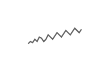
\begin{tikzpicture}[x=0.08em, y=0.08em, line width=0.4pt]
                \draw[FooterGray] (0,3) -- (1,4) -- (2,3.5) -- (3,5) -- (4,4) -- (5,6) -- (6,5.5) -- (7,4) -- (8,5) -- (9,7) -- (10,6) -- (11,5) -- (12,6.5) -- (13,8) -- (14,7) -- (15,6) -- (16,7.5) -- (17,9) -- (18,8) -- (19,7) -- (20,8.5) -- (21,10) -- (22,9) -- (23,8) -- (24,9.5);
            \end{tikzpicture}%
        }%
        \hskip0.5cm%
    }%
    \vskip6pt%
}

%=============================================================================
% PACHETE
%=============================================================================
\usepackage[utf8]{inputenc}
\usepackage[T1]{fontenc}
\usepackage{amsmath, amssymb, amsthm}
\usepackage{mathtools}
\usepackage{bm}
\usepackage{tikz}
\usetikzlibrary{arrows.meta, positioning, shapes, calc, decorations.pathreplacing, shadings}
\usepackage{booktabs}
\usepackage{multirow}
\usepackage{array}
\usepackage{graphicx}
\usepackage{hyperref}
\usepackage{colortbl}
\usepackage{pifont}
\hypersetup{colorlinks=true, linkcolor=MainBlue, urlcolor=MainBlue}
\graphicspath{{../../logos/}{../../charts/}{../../photos/}}
\hfuzz=2pt  % Suppress tiny overfull warnings (<2pt)
\vfuzz=2pt  % Suppress tiny vertical overfull warnings (<2pt)

%=============================================================================
% COMANDA QUANTLET
%=============================================================================
\newcommand{\quantlet}[2]{%
    \vspace{-0.25cm}%
    \hfill\href{#2}{%
        \raisebox{-0.15em}{
\includegraphics[height=0.7em]{ql_logo.png}}%
        \textcolor{MainBlue}{\tiny\ #1}%
    }\par%
}

%=============================================================================
% PAGINĂ TITLU PERSONALIZATĂ
%=============================================================================
\defbeamertemplate*{title page}{hybrid}[1][]
{
    \vspace{0.2cm}
    % Rând logo-uri - antet superior (cu linkuri clickabile)
    \begin{center}
        \href{https://www.ase.ro}{
\includegraphics[height=1.0cm]{ase_logo.png}}\hspace{0.3cm}%
        \href{https://theida.net}{
\includegraphics[height=1.0cm]{ida_logo.png}}\hspace{0.3cm}%
        \href{https://blockchain-research-center.com}{
\includegraphics[height=1.0cm]{brc_logo.png}}\hspace{0.3cm}%
        \href{https://www.ai4efin.ase.ro}{
\includegraphics[height=1.0cm]{ai4efin_logo.png}}\hspace{0.3cm}%
        \href{https://ipe.ro/new}{
\includegraphics[height=1.0cm]{acad_logo.png}}\hspace{0.3cm}%
        \href{https://www.digital-finance-msca.com}{
\includegraphics[height=1.0cm]{msca_logo.png}}%
    \end{center}

    \vspace{0.6cm}

    % Titlu principal cu logo-uri Q pe părți (cu linkuri clickabile)
    \begin{center}
        \begin{minipage}{0.1\textwidth}
            \centering
            \href{https://quantlet.com}{
\includegraphics[height=1.1cm]{ql_logo.png}}
        \end{minipage}%
        \begin{minipage}{0.78\textwidth}
            \centering
            {\LARGE\bfseries\usebeamercolor[fg]{title}\inserttitle}

            \vspace{0.3cm}

            {\usebeamerfont{subtitle}\usebeamercolor[fg]{title}\insertsubtitle}
        \end{minipage}%
        \begin{minipage}{0.1\textwidth}
            \centering
            \href{https://quantinar.com}{
\includegraphics[height=1.1cm]{qr_logo.png}}
        \end{minipage}
    \end{center}

    \vspace{0.6cm}

    % Autori (aliniere la stânga)
    \hspace{0.5cm}\begin{minipage}[t]{0.9\textwidth}
        \usebeamerfont{author}\insertauthor
    \end{minipage}

    \vspace{0.3cm}

    % Institut/Afilieri (aliniere la stânga)
    \hspace{0.5cm}\begin{minipage}[t]{0.9\textwidth}
        \raggedright\small\insertinstitute
    \end{minipage}
}

%=============================================================================
% MEDII PENTRU TEOREME
%=============================================================================
\theoremstyle{definition}
\setbeamertemplate{theorems}[numbered]
\newtheorem{defn}{Definiție}
\newtheorem{thm}{Teoremă}
\newtheorem{prop}{Propoziție}
\newtheorem{rmk}{Observație}

%=============================================================================
% CENTRED MINIPAGE
%=============================================================================
\newenvironment{cminipage}[1]{%
    \par\noindent\hfill\begin{minipage}{#1}\ignorespaces
}{%
    \end{minipage}\hfill\null\par
}

%=============================================================================
% COMENZI PERSONALIZATE
%=============================================================================
\newcommand{\E}{\mathbb{E}}
\newcommand{\Var}{\text{Var}}
\newcommand{\Cov}{\text{Cov}}
\newcommand{\Corr}{\text{Corr}}
\newcommand{\R}{\mathbb{R}}
\newcommand{\N}{\mathbb{N}}
\newcommand{\Z}{\mathbb{Z}}
\newcommand{\B}{\mathbf{B}}
\newcommand{\imark}{\textcolor{MainBlue}{\textbullet}}
\newcommand{\RMSE}{\text{RMSE}}
\newcommand{\MAE}{\text{MAE}}
\newcommand{\MAPE}{\text{MAPE}}

% Indicatoare nivel academic pe slide-uri  (numeric \ifnum — bulletproof in beamer templates)
\newcount\slidelevelnum
\global\slidelevelnum=0
\makeatletter
\newcommand{\slidelevel}[1]{%
    \global\slidelevelnum=0%
    \def\tmp@SL{#1}\def\tmp@SLy{Y3}\def\tmp@SLm{MSc}\def\tmp@SLp{PhD}%
    \ifx\tmp@SL\tmp@SLy \global\slidelevelnum=1\fi%
    \ifx\tmp@SL\tmp@SLm \global\slidelevelnum=2\fi%
    \ifx\tmp@SL\tmp@SLp \global\slidelevelnum=3\fi%
}
\makeatother
\gdef\currentlevelcolor{FooterGray}
\newcommand{\showlevel}{%
    \ifnum\slidelevelnum=1%
        \colorbox{Forest}{\strut\textcolor{white}{\sffamily\bfseries\fontsize{8}{9}\selectfont Y3}}%
        \gdef\currentlevelcolor{Forest}%
    \fi%
    \ifnum\slidelevelnum=2%
        \colorbox{MainBlue}{\strut\textcolor{white}{\sffamily\bfseries\fontsize{8}{9}\selectfont MSc}}%
        \gdef\currentlevelcolor{MainBlue}%
    \fi%
    \ifnum\slidelevelnum=3%
        \colorbox{Crimson}{\strut\textcolor{white}{\sffamily\bfseries\fontsize{8}{9}\selectfont PhD}}%
        \gdef\currentlevelcolor{Crimson}%
    \fi%
    \ifnum\slidelevelnum=0%
        \gdef\currentlevelcolor{FooterGray}%
    \fi%
}


%=============================================================================
% INFORMATII TITLU
%=============================================================================
\title[Statistica Piețelor Financiare]{Statistica Piețelor Financiare}
\subtitle{Capitolul 2: Distribuții clasice și fapte stilizate}
\author[D.T. Pele, A. Amza]{\texorpdfstring{\begin{tabular}[t]{@{}l@{}}Daniel Traian PELE \\ Antoaneta Amza\end{tabular}}{Daniel Traian PELE, Antoaneta Amza}}
\institute{Academia de Studii Economice din București\\
IDA Institute Digital Assets\\
Blockchain Research Center\\
AI4EFin Artificial Intelligence for Energy Finance\\
Academia Română, Institutul de Prognoză Economică\\
MSCA Digital Finance}
\date{}

\begin{document}

% Pagina de titlu (fara antet/subsol)
{
\setbeamertemplate{headline}{}
\setbeamertemplate{footline}{}
\begin{frame}
    \titlepage
\end{frame}
}

%=============================================================================
% OBIECTIVE DE INVATARE
%=============================================================================
\begin{frame}{Obiective de învățare}
    \begin{block}{La sfârșitul acestui curs, veți fi capabili să:}
    \begin{enumerate}
        \item[\textcolor{MainBlue}{\textbf{1.}}] \textbf{Explicați} de ce alegerea distribuției afectează estimarea riscului financiar
        \item[\textcolor{MainBlue}{\textbf{2.}}] \textbf{Calculați} log-randamente și interpretați proprietățile lor statistice
        \item[\textcolor{MainBlue}{\textbf{3.}}] \textbf{Aplicați} teste de normalitate și interpretați rezultatele
        \item[\textcolor{MainBlue}{\textbf{4.}}] \textbf{Identificați} faptele stilizate ale randamentelor financiare
        \item[\textcolor{MainBlue}{\textbf{5.}}] \textbf{Ajustați} distribuția Student-$t$ și comparați cu distribuția normală
    \end{enumerate}
    \end{block}
\end{frame}

%=============================================================================
% CUPRINS
%=============================================================================
{
\setbeamertemplate{headline}{%
    \vskip10pt%
    \hbox to \paperwidth{\hskip0.5cm\hfill\hskip0.5cm}%
    \vskip4pt%
    {\color{FooterGray}\hrule height 0.4pt}%
}
\begin{frame}{}
    {\color{FooterGray}\hrule height 0.4pt}
    \vspace{0.1cm}
    {\Large\textcolor{IDAred}{\textbf{Cuprins}}}
    \vspace{0.2cm}
    {\small
    \begin{itemize}
        \item Introducere --- De ce contează distribuțiile
        \item De la prețuri la log-randamente
        \item Distribuția normală
        \item Fapte stilizate ale randamentelor financiare
        \item Distribuția Student-$t$
        \item Distribuția Pareto
    \end{itemize}
    }
\end{frame}
}
%=============================================================================
% SECȚIUNEA 1: INTRODUCERE
%=============================================================================
\section{Introducere --- De ce contează distribuțiile}

%--- Y3 Slide 1 ---
\slidelevel{Y3}
\begin{frame}{De ce contează alegerea distribuției?}
\begin{itemize}
\item Dacă presupunem o distribuție greșită, \textbf{subestimăm} probabilitatea pierderilor extreme
\item \textbf{Exemplu}: 19 octombrie 1987 --- S\&P~500 a scăzut cu 20{,}5\% într-o singură zi
\begin{itemize}
\item Sub ipoteza normală ($\sigma \approx 1\%$): un eveniment de $\sim$20$\sigma$ cu probabilitate $\approx 10^{-89}$
\item Și totuși s-a întâmplat --- distribuția normală este inadecvată pentru evenimente extreme
\end{itemize}
\item Băncile și autoritățile de reglementare trebuie să cuantifice ,,cât de rău poate fi?''
\item Acest lucru necesită \textbf{modele distribuționale precise}
\end{itemize}

\vspace{0.3cm}
\begin{alertblock}{Idee cheie}
\begin{itemize}
\item Alegerea distribuției de probabilitate determină direct cât capital trebuie să dețină o bancă pentru acoperirea pierderilor potențiale
\end{itemize}
\end{alertblock}
\end{frame}

%--- Y3 Slide 2 ---
\slidelevel{Y3}
\begin{frame}{Problema alegerii distribuției}
\begin{itemize}
\item \textbf{Anticipare}: Mai târziu vom defini formal \textbf{Value-at-Risk (VaR)}, o măsură cheie de risc care depinde complet de ipoteza distribuțională
\item Candidații pe care îi vom studia:
\begin{itemize}
\item \textbf{Normală} --- referința clasică (cozi subțiri)
\item \textbf{Student-$t$} --- cozi mai groase, momente superioare finite
\item \textbf{Stabilă} --- cele mai groase cozi, varianță infinită (\textit{infinite variance}) posibilă
\item \textbf{EVT} --- modelează doar cozile, agnostică față de centru
\end{itemize}
\item Fiecare model implică un răspuns diferit la ,,cât de rău poate fi?''
\end{itemize}

\vspace{0.2cm}
\begin{center}
\renewcommand{\arraystretch}{1.1}
\begin{tabular}{lccc}
\toprule
\textbf{Model} & \textbf{Tip coadă} & \textbf{Kurtosis} & \textbf{Parametri} \\
\midrule
Normal & Exponențială & 3 & 2 \\
Student-$t$ & Lege putere & $>3$ & 3 \\
Stabilă & Lege putere & $\infty$ & 4 \\
GPD (EVT) & Flexibilă & --- & 2 \\
\bottomrule
\end{tabular}
\end{center}
\end{frame}

%--- Y3 Slide 3 ---
\slidelevel{Y3}
\begin{frame}{Structura capitolului}
\begin{columns}[T]
\begin{column}{0.48\textwidth}
\begin{block}{Fundamente}
\begin{enumerate}
\item De la prețuri la log-randamente
\item Distribuția normală (referință)
\item Fapte stilizate ale randamentelor
\item Distribuția Student-$t$
\item Distribuții asimetrice
\end{enumerate}
\end{block}
\end{column}
\begin{column}{0.48\textwidth}
\begin{block}{Modele avansate și aplicații}
\begin{enumerate}\setcounter{enumi}{5}
\item Distribuții stabile
\item Teoria Valorilor Extreme
\item Compararea distribuțiilor
\item \textcolor{Crimson}{\textbf{Managementul riscului (VaR, ES)}}
\item Extensii moderne (GARCH)
\end{enumerate}
\end{block}
\end{column}
\end{columns}

\end{frame}

%--- MSc Slide 4 ---
\slidelevel{MSc}
\begin{frame}{Alegerea distribuției și evaluarea instrumentelor financiare derivate}
\begin{itemize}
\item Black--Scholes presupune log-normalitate $\Rightarrow$ volatilitate implicită constantă
\item Deviațiile empirice produc \textbf{zâmbetul/asimetria volatilității (\textit{volatility smile/skew})}
\item Optimizarea portofoliului sub randamente non-Gaussiene: medie-varianță este suboptimală
\item Context de reglementare: Basel~II $\to$ Basel~III/IV
\begin{itemize}
\item Basel~II: VaR 1\% cu ipoteză normală
\item Basel~III/IV: trecerea de la VaR 1\% la ES 2{,}5\%
\end{itemize}
\end{itemize}

\vspace{0.3cm}
\begin{rmk}
\begin{itemize}
\item Întregul cadru Basel de capital de reglementare se bazează pe ipoteze distribuționale
\item Subestimarea riscului de coadă $\Rightarrow$ capital insuficient $\Rightarrow$ fragilitate sistemică
\end{itemize}
\end{rmk}
\end{frame}

%--- Y3 Slide 4b ---
\slidelevel{Y3}
\begin{frame}{S\&P 500: cum arată lumea reală}
\vspace{-0.3cm}
\begin{center}
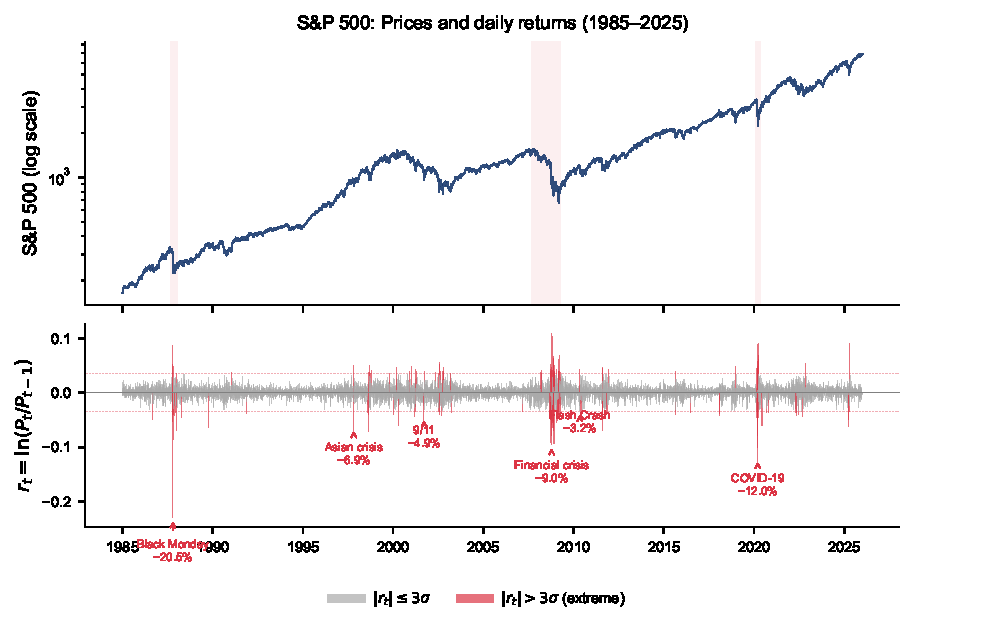
\includegraphics[width=0.60\textwidth]{ch2_sp500_history.pdf}
\end{center}
\vspace{-0.4cm}
\quantlet{SFM\_ch2\_stylized\_facts}{https://github.com/QuantLet/Stat_fin_markets/tree/master/Ch_02/SFM_ch2_stylized_facts}
\vspace{-0.3cm}
\begin{itemize}
\item Crahurile ($|r_t| > 3\sigma$) apar mult mai frecvent decât prevede distribuția normală
\item Randamentele extreme se \textbf{clusterizează}; avem nevoie de modele cu cozi groase (\textit{heavy tails})
\end{itemize}
\end{frame}

%--- PhD Slide 5 ---
\slidelevel{PhD}
\begin{frame}{Incertitudinea modelului și măsuri robuste de risc}
\begin{itemize}\setlength\itemsep{2pt}
\item \textbf{Incertitudinea modelului}: Care distribuție este ,,corectă''? Poate niciuna --- orice model este o \emph{aproximare}.
\item \textbf{Aversiune față de ambiguitate} (paradoxul Ellsberg): decidentul nu cunoaște distribuția exactă și adoptă o atitudine conservatoare.
\item Măsuri robuste de risc sub incertitudine distribuțională:
\[
\rho_{\text{robust}}(X) = \sup_{Q \in \mathcal{Q}} \rho_Q(X)
\]
\item \textbf{Mulțimea de ambiguitate} $\mathcal{Q}$ = o mulțime de distribuții de probabilitate considerate plauzibile. Se calculează riscul sub \emph{cea mai defavorabilă} distribuție din $\mathcal{Q}$ (\textit{worst-case}).
\item Exemple clasice de $\mathcal{Q}$:
\begin{itemize}
    \item \textbf{Bazată pe momente}: toate distribuțiile cu $(\mu, \sigma^2)$ date: $\mathcal{Q} = \{Q : \E_Q[X] = \mu,\; \Var_Q(X) = \sigma^2\}$
    \item \textbf{Wasserstein}: vecinătate de rază $\varepsilon$ în jurul distribuției empirice: $\mathcal{Q} = \{Q : W_p(Q, \hat{P}_n) \leq \varepsilon\}$
    \item \textbf{KL-divergență}: $\mathcal{Q} = \{Q : D_{\text{KL}}(Q \| P_0) \leq \eta\}$
\end{itemize}
\item \textbf{Cuantificarea riscului de model}: intervalul VaR/ES între modele plauzibile furnizează o ,,primă de risc de model''
\end{itemize}
\end{frame}

%--- PhD Slide 5b ---
\slidelevel{PhD}
\begin{frame}{Distanțe între distribuții --- Intuiție}
\begin{itemize}\setlength\itemsep{3pt}
\item \textbf{Problema}: Cum măsurăm cât de ,,aproape'' sunt două distribuții $P$ și $Q$?
\item \textbf{Distanța Wasserstein} $W_p(P, Q)$:
\begin{itemize}
    \item Cunoscută și ca \textit{Earth Mover's Distance} (distanța mutării de pământ)
    \item Intuiție: costul minim de ,,transport'' al masei de probabilitate din $P$ în $Q$
    \item Dacă $P$ și $Q$ sunt distribuții pe $\R$ cu CDF-uri $F_P, F_Q$:
    \[
    W_1(P, Q) = \int_{-\infty}^{+\infty} |F_P(x) - F_Q(x)|\, dx
    \]
    \item Avantaj: ține cont de \emph{geometria} spațiului (nu doar de suprapunerea densităților)
\end{itemize}
\item \textbf{Divergența Kullback--Leibler} $D_{\text{KL}}(Q \| P_0)$:
\begin{itemize}
    \item Măsoară ,,pierderea de informație'' dacă aproximăm $Q$ prin $P_0$
    \item $D_{\text{KL}}(Q \| P_0) = \int q(x) \ln \frac{q(x)}{p_0(x)}\, dx \geq 0$, cu egalitate iff $Q = P_0$
    \item \textbf{Nu} este o distanță propriu-zisă (nu este simetrică: $D_{\text{KL}}(Q\|P) \neq D_{\text{KL}}(P\|Q)$)
\end{itemize}
\item \textbf{Aplicație}: Alegerea razei $\varepsilon$ (Wasserstein) sau $\eta$ (KL) controlează \emph{gradul de conservatorism} al măsurii robuste de risc --- $\varepsilon$ mare $\Rightarrow$ mulțime $\mathcal{Q}$ mai largă $\Rightarrow$ VaR robust mai mare
\end{itemize}
\end{frame}

%--- Y3 Slide 6 ---
\slidelevel{Y3}
\begin{frame}{Distribuția normală vs.\ realitate --- Vizualizare și exemplu}
\begin{columns}[T]
\begin{column}{0.50\textwidth}
\begin{center}
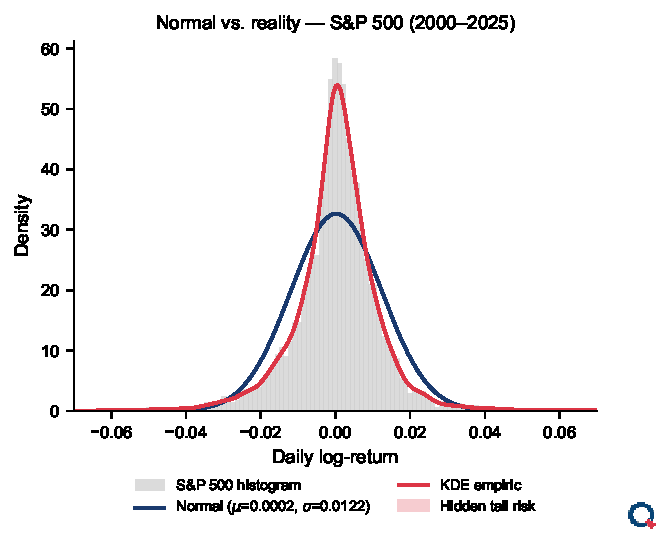
\includegraphics[width=0.92\linewidth]{ch2_normal_vs_empirical.pdf}
\end{center}
\vspace{-0.2cm}
\quantlet{SFM\_ch2\_normal\_distribution}{https://github.com/QuantLet/Stat_fin_markets/tree/master/Ch_02/SFM_ch2_normal_distribution}
\end{column}
\begin{column}{0.46\textwidth}
\begin{exampleblock}{\small Black Monday --- 19 oct.\ 1987}
{\small S\&P~500 a scăzut cu $20{,}5\%$ într-o zi.}
\begin{itemize}\setlength{\itemsep}{0pt}
\item {\small Normală: $\sim$20$\sigma$, $P \approx 10^{-89}$}
\item {\small Student-$t$ ($\nu\!=\!4$): $P \approx 10^{-5}$}
\end{itemize}
\end{exampleblock}
\vspace{-0.15cm}
\begin{alertblock}{\small Timpul de revenire}
{\small $T = \tfrac{1}{252 \times 10^{-89}} \approx 4 \times 10^{86}$ ani;
vârsta universului: $\approx 1{,}4 \times 10^{10}$ ani\\[1pt]
\textbf{$\Rightarrow$ $\boldsymbol{\sim 10^{76}}$ vârste ale universului!}}
\end{alertblock}
\end{column}
\end{columns}
\end{frame}

%=============================================================================
% SECȚIUNEA 2: DE LA PREȚURI LA LOG-RANDAMENTE
%=============================================================================
\section{De la prețuri la log-randamente}

%--- Y3 Slide 1 ---
\slidelevel{Y3}
\begin{frame}{Definiția log-randamentelor}
\begin{defn}[Log-randament]
\textbf{Log-randamentul} (randamentul compus continuu) la momentul $t$ este:
\[
r_t = \ln\!\left(\frac{P_t}{P_{t-1}}\right) = \ln P_t - \ln P_{t-1}
\]
unde $P_t$ este prețul activului la momentul $t$.
\end{defn}

\vspace{0.2cm}
\begin{itemize}
\item \textbf{Aditivitate}: Randamentele multi-perioadă sunt sume: $r_{t:t+k} = \sum_{i=1}^{k} r_{t+i}$
\item \textbf{Aproximare}: Pentru randamente mici, $r_t \approx (P_t - P_{t-1})/P_{t-1}$
\item \textbf{Motivație statistică}: Structura aditivă permite teoria probabilităților standard (TLC, limite stabile)
\end{itemize}

\end{frame}

%--- Y3 Slide 2 ---
\slidelevel{Y3}
\begin{frame}{Proprietățile log-randamentelor}
\begin{columns}[T]
\begin{column}{0.48\textwidth}
\begin{block}{De ce log-randamente?}
\begin{itemize}
\item Aditive în timp: $r_{[0,T]} = \sum_{t=1}^{T} r_t$
\item Simetrice: $+5\%$ și $-5\%$ sunt comparabile
\item Nemărginite inferior: pot modela pierderi mari
\item Permit inferență bazată pe TLC
\end{itemize}
\end{block}
\end{column}
\begin{column}{0.48\textwidth}
\begin{block}{Randamente simple vs.\ log-randamente}
\begin{itemize}
\item Randament simplu: $R_t = \frac{P_t - P_{t-1}}{P_{t-1}}$
\item Relație: $r_t = \ln(1 + R_t)$
\item Randamentele simple \textit{nu} sunt aditive în timp
\item Dar \textit{sunt} aditive pe activele din portofoliu
\end{itemize}
\end{block}
\end{column}
\end{columns}

\vspace{0.3cm}
\begin{exampleblock}{Convenție}
\begin{itemize}
\item Pe parcursul acestui capitol, $r_t$ denotă \textbf{log-randamentul}, dacă nu se specifică altfel
\end{itemize}
\end{exampleblock}
\end{frame}

%--- MSc Slide 3 ---
\slidelevel{MSc}
\begin{frame}{Limita în timp continuu}
\begin{itemize}
\item Mișcarea Browniană geometrică: $dS/S = \mu\,dt + \sigma\,dW$
\item Prin lema lui It\^{o}: $d\ln S = (\mu - \sigma^2/2)\,dt + \sigma\,dW$
\item Inegalitatea lui Jensen: $\E[\ln(P_T/P_0)] \neq \ln(\E[P_T/P_0])$
\begin{itemize}
\item Randamentul mediu aritmetic depășește randamentul mediu geometric
\item Diferența $\approx \sigma^2/2$ (,,pierderea din volatilitate (\textit{volatility drag})'')
\end{itemize}
\item Log-randamente: aditive în \textit{timp}; randamente simple: aditive pe \textit{active}
\end{itemize}

\vspace{-0.2cm}
\begin{center}
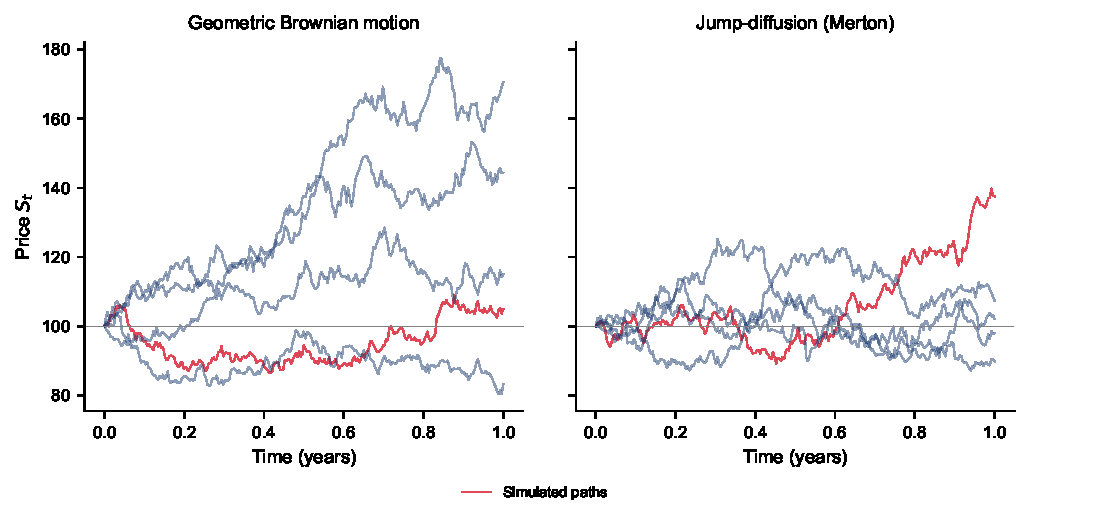
\includegraphics[width=0.45\textwidth]{ch2_gbm_vs_levy.pdf}
\end{center}
\quantlet{SFM\_ch2\_distribution\_comparison}{https://github.com/QuantLet/Stat_fin_markets/tree/master/Ch_02/SFM_ch2_distribution_comparison}
\end{frame}

%--- PhD Slide 4 ---
\slidelevel{PhD}
\begin{frame}{Reprezentarea semimartingală}
\begin{itemize}
\item Procesele de preț modelate ca \textbf{semimartingale}: $S_t = S_0 + A_t + M_t$
\item Lema lui It\^{o} pentru semimartingale cu salturi:
\[
d\ln S_t = \frac{dS_t}{S_{t^-}} - \frac{1}{2}\frac{d[S,S]_t^c}{S_{t^-}^2} + \sum_{s \leq t}\left(\ln\frac{S_s}{S_{s^-}} - \frac{\Delta S_s}{S_{s^-}}\right)
\]
\item Variația cuadratică și volatilitatea realizată:
\[
[X,X]_t = \lim_{\|\Pi\| \to 0} \sum_{i} (X_{t_{i+1}} - X_{t_i})^2
\]
\item Procese de preț discontinue: salturi și descompunerea L\'{e}vy--It\^{o}
\end{itemize}
\end{frame}

%--- Y3 Slide 5 ---
\slidelevel{Y3}
\begin{frame}{Exemplu numeric: Calculul log-randamentelor}
\begin{exampleblock}{Exercițiu}
Prețuri: $P_0\!=\!100$, $P_1\!=\!103$, $P_2\!=\!101$, $P_3\!=\!105$, $P_4\!=\!102$. Calculați log-randamentele, media și varianța.
\end{exampleblock}
\vspace{-0.1cm}
\begin{block}{Rezolvare}
\begin{center}
\renewcommand{\arraystretch}{1.0}
\small
\begin{tabular}{cccccc}
\toprule
$t$ & $P_t$ & $R_t$ & $r_t$ & $r_t - \bar{r}$ & $(r_t - \bar{r})^2$ \\
\midrule
1 & 103 & $+3{,}00\%$ & $+2{,}96\%$ & $2{,}46\%$ & $0{,}0605\%$ \\
2 & 101 & $-1{,}94\%$ & $-1{,}96\%$ & $-2{,}46\%$ & $0{,}0605\%$ \\
3 & 105 & $+3{,}96\%$ & $+3{,}88\%$ & $3{,}38\%$ & $0{,}1143\%$ \\
4 & 102 & $-2{,}86\%$ & $-2{,}90\%$ & $-3{,}40\%$ & $0{,}1153\%$ \\
\midrule
\multicolumn{3}{l}{$\bar{r} = 0{,}495\%$} & \multicolumn{3}{l}{$s^2 = \frac{\sum(r_t - \bar{r})^2}{3} = 0{,}1169\%$} \\
\bottomrule
\end{tabular}
\end{center}
\begin{itemize}
\item \textbf{Aditivitate}: $r_{[0,4]} = \ln(102/100) = 1{,}98\% = \sum_{t=1}^{4} r_t$ \checkmark
\end{itemize}
\end{block}
\end{frame}

%=============================================================================
% SECȚIUNEA 3: DISTRIBUȚIA NORMALĂ
%=============================================================================
\section{Distribuția normală}

%--- Y3 Slide 1 ---
\slidelevel{Y3}
\begin{frame}{Distribuția normală --- Definiție și proprietăți}
\begin{defn}[Distribuția normală]
$X \sim N(\mu, \sigma^2)$ dacă:
\[
f(x) = \frac{1}{\sigma\sqrt{2\pi}}\exp\!\left(-\frac{(x-\mu)^2}{2\sigma^2}\right), \quad x \in \R.
\]
\end{defn}

\begin{columns}[T]
\begin{column}{0.48\textwidth}
\begin{block}{Momente}
\begin{itemize}
\item $\E[X] = \mu$, \quad $\Var(X) = \sigma^2$
\item Asimetrie $= 0$
\item Kurtosis $= 3$ (exces de kurtosis $= 0$)
\end{itemize}
\end{block}
\end{column}
\begin{column}{0.48\textwidth}
\begin{block}{Proprietăți cheie}
\begin{itemize}
\item Simetrică față de $\mu$
\item Regula 68--95--99{,}7
\item Cozile scad ca $e^{-x^2/2}$
\end{itemize}
\end{block}
\end{column}
\end{columns}
\end{frame}

%--- Y3 Slide 1b ---
\slidelevel{Y3}
\begin{frame}{Distribuția normală --- Graficul densității}
\begin{center}
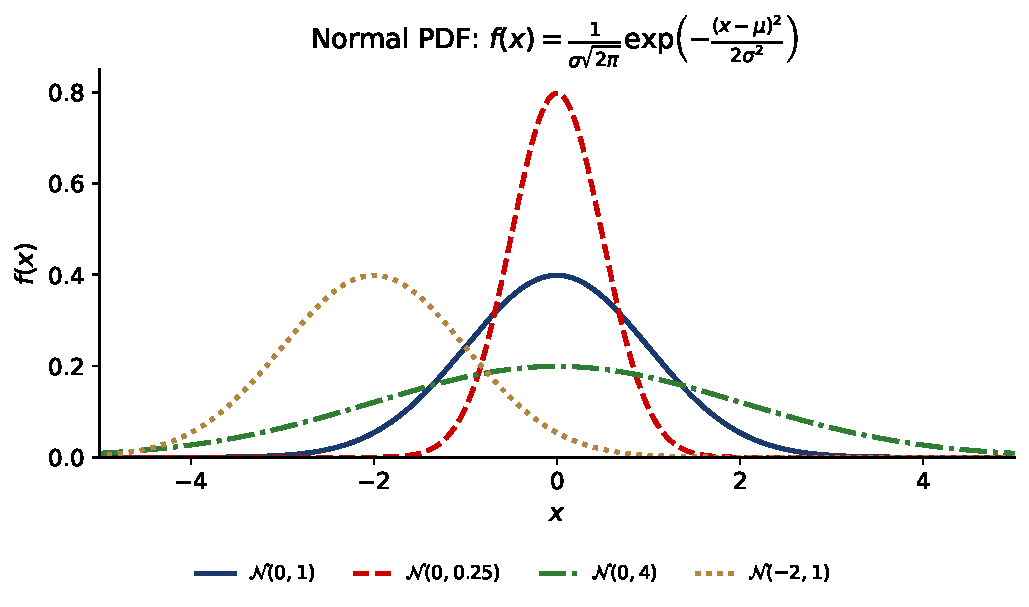
\includegraphics[width=0.52\textwidth]{ch2_normal_pdf_theoretical.pdf}
\end{center}
\vspace{-0.2cm}
\quantlet{SFM\_ch2\_normal\_distribution}{https://github.com/QuantLet/Stat_fin_markets/tree/master/Ch_02/SFM_ch2_normal_distribution}
\vspace{-0.1cm}
\begin{itemize}
\item Forma de \textbf{clopot}: simetrică, unimodală, maximă în $x = \mu$
\item Parametrii $\mu$ și $\sigma^2$ controlează \textbf{poziția} și \textbf{dispersia}
\item Cozile scad \textbf{exponențial}: $f(x) \sim e^{-x^2/2}$ --- subestimează evenimentele extreme
\end{itemize}
\end{frame}

%--- Y3 Slide 2 ---
\slidelevel{Y3}
\begin{frame}{Cuantile și Teorema Limită Centrală}
\begin{itemize}
\item \textbf{Cuantile}: Cuantila de ordin $\alpha$ a $N(\mu, \sigma^2)$ este:
\[
q_\alpha = \mu + \sigma\,\Phi^{-1}(\alpha)
\]
Aceasta va fi utilizată pentru a defini Value-at-Risk
\item \textbf{Cuantile cheie}: $\Phi^{-1}(0{,}01) = -2{,}326$, \quad $\Phi^{-1}(0{,}05) = -1{,}645$
\end{itemize}

\vspace{0.2cm}
\begin{thm}[Teorema Limită Centrală]
Dacă $X_1, X_2, \ldots$ sunt i.i.d.\ cu $\E[X_i] = \mu$ și $\Var(X_i) = \sigma^2 < \infty$, atunci:
\[
\frac{\bar{X}_n - \mu}{\sigma/\sqrt{n}} \xrightarrow{d} N(0,1).
\]
\end{thm}

\begin{itemize}
\item \textbf{Stabilitate}: Suma unor v.a.\ independente distribuite normal este normală: $X + Y \sim N(\mu_1+\mu_2, \sigma_1^2+\sigma_2^2)$
\end{itemize}
\end{frame}

%--- Y3 Slide 3 ---
\slidelevel{Y3}
\begin{frame}{Ilustrarea TLC}
\begin{center}
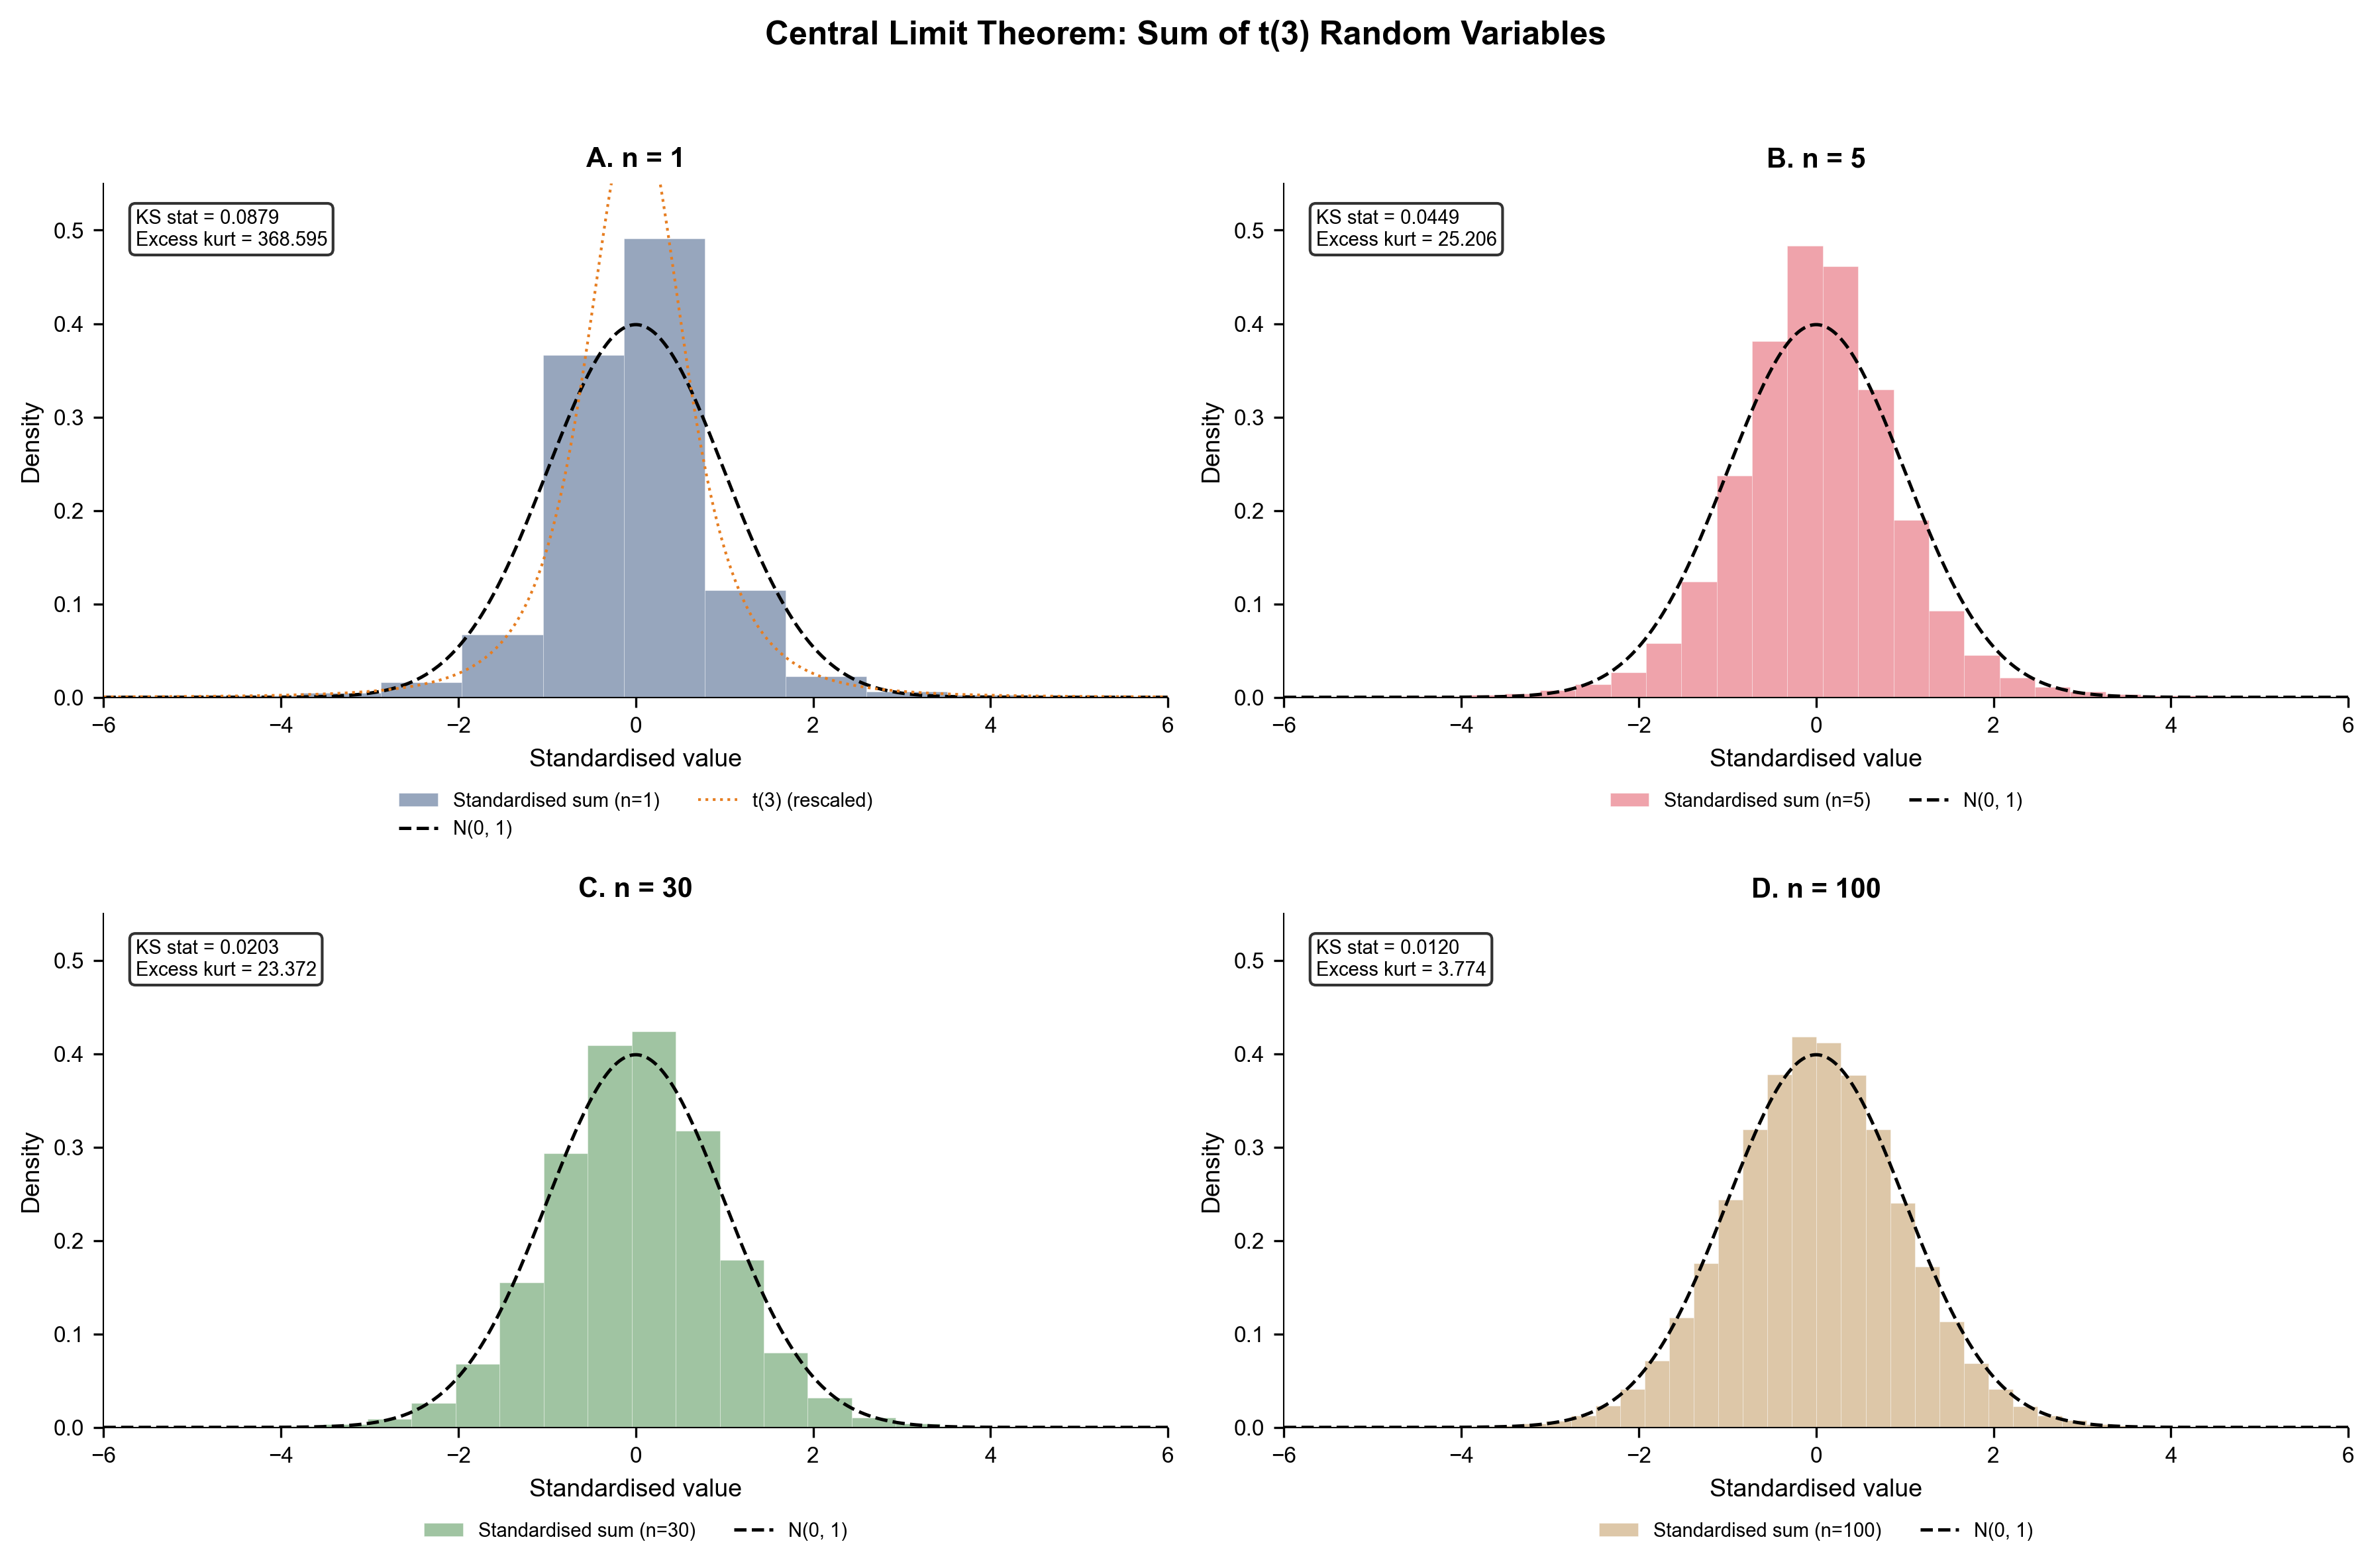
\includegraphics[width=0.50\textwidth]{ch2_clt_illustration.png}
\end{center}
\vspace{-0.2cm}
\quantlet{SFM\_ch2\_normal\_distribution}{https://github.com/QuantLet/Stat_fin_markets/tree/master/Ch_02/SFM_ch2_normal_distribution}
\vspace{-0.1cm}
\begin{itemize}
\item Pe măsură ce $n$ crește, $\bar{X}_n$ se apropie de normalitate
\item \textbf{Limitare}: TLC necesită varianță finită --- ce se întâmplă dacă $\sigma^2 = \infty$?
\end{itemize}
\end{frame}

%--- Y3 Slide 4 ---
\slidelevel{Y3}
\begin{frame}{Ajustarea normală pe randamentele S\&P 500}
\begin{center}
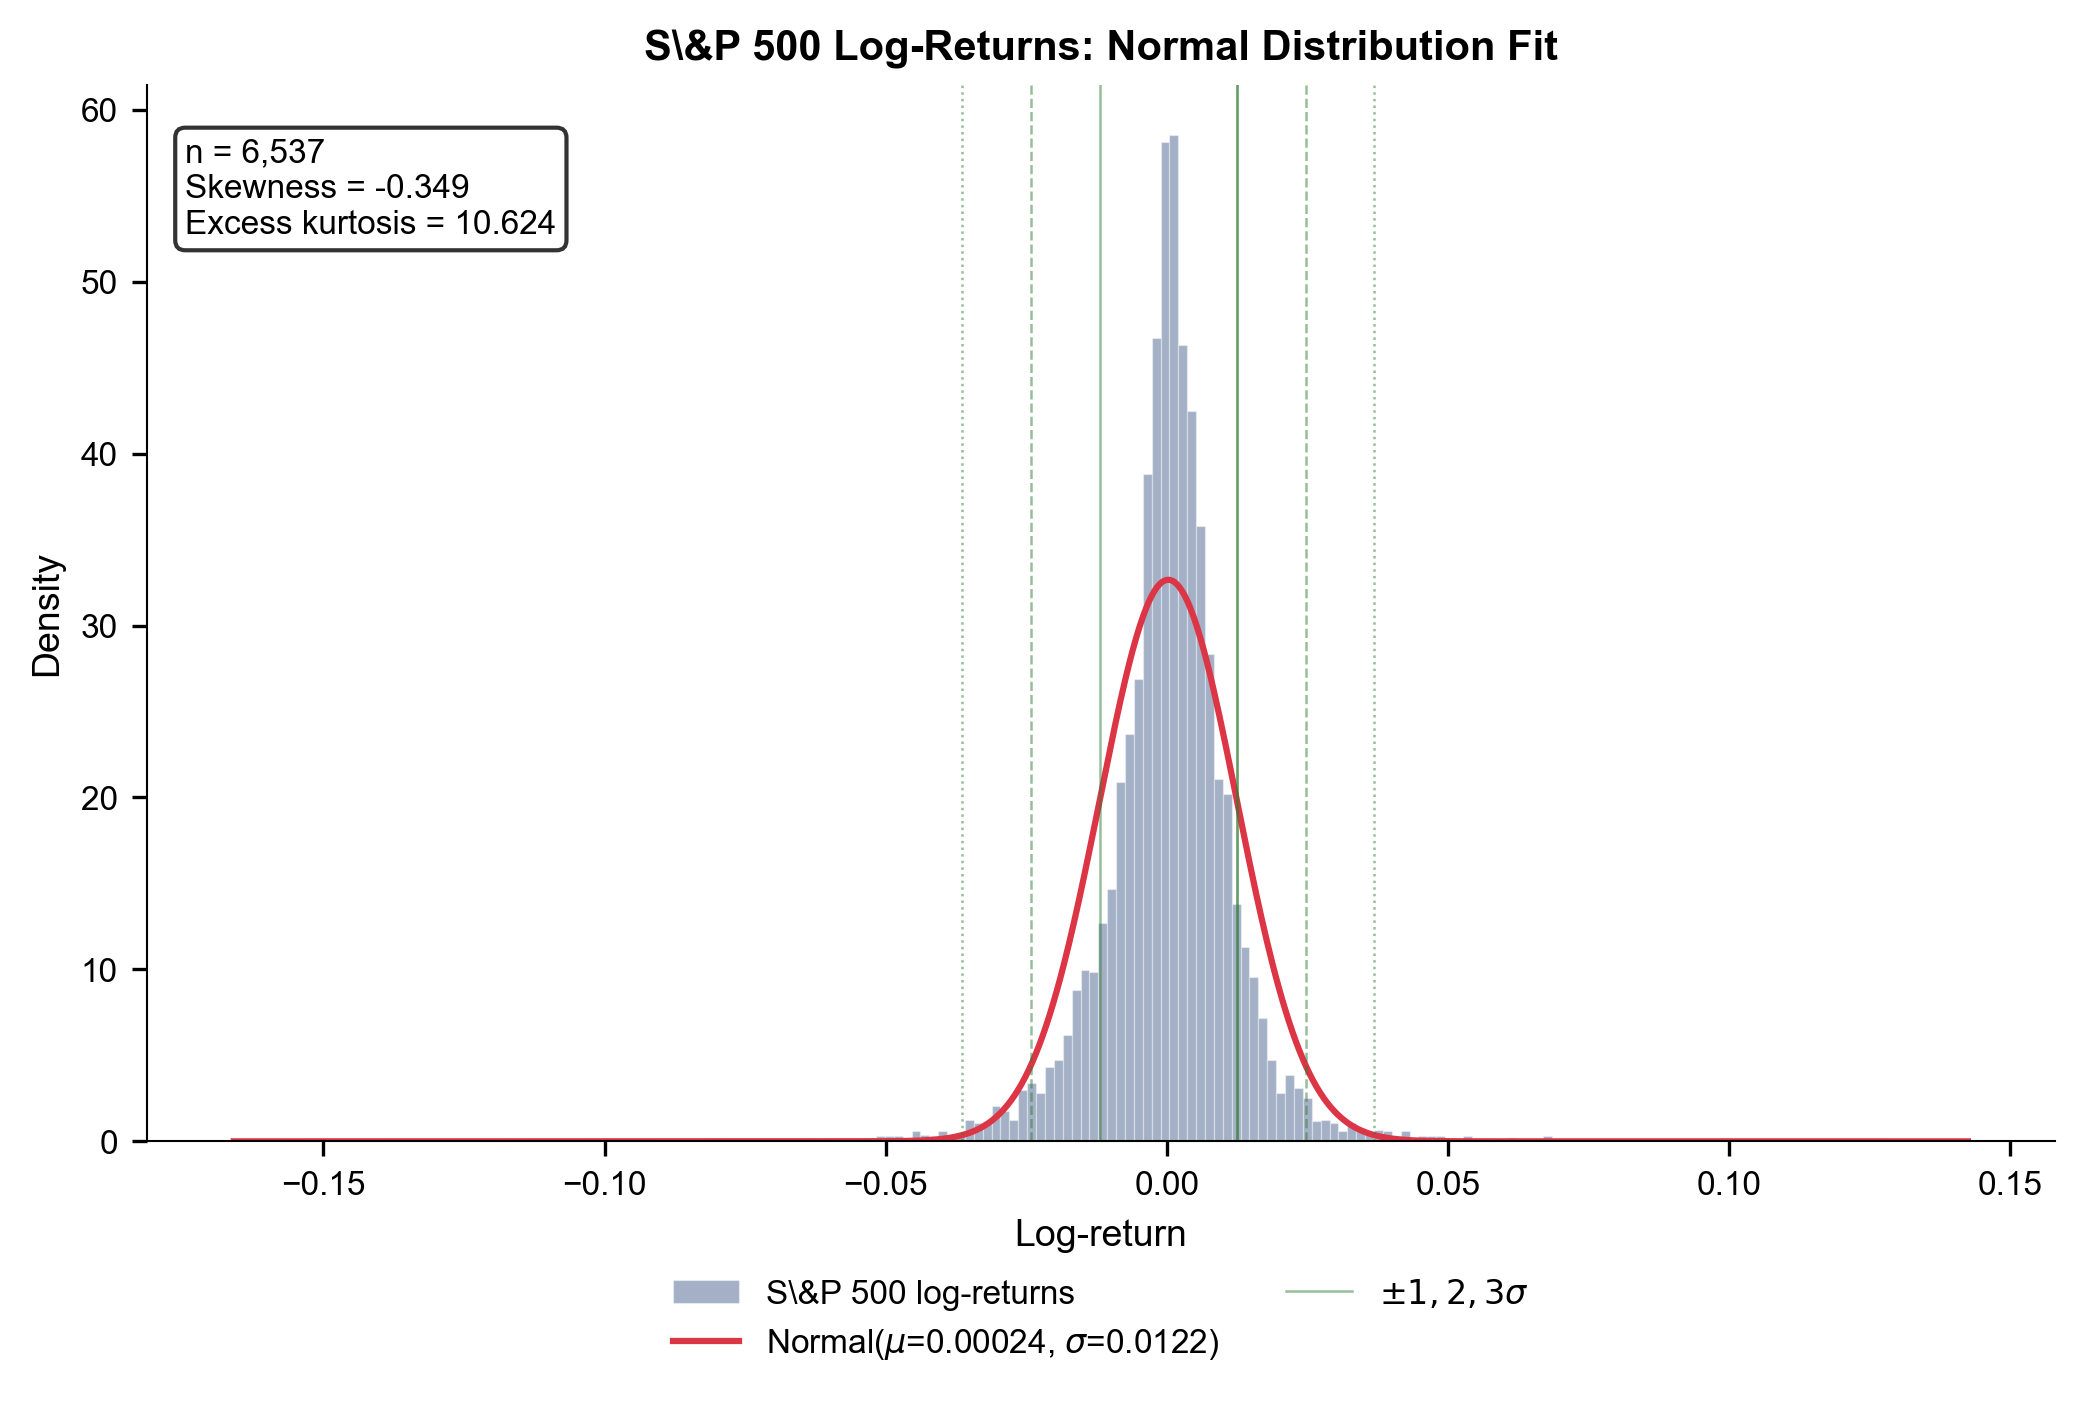
\includegraphics[width=0.5\textwidth]{ch2_normal_fit.png}
\end{center}
\quantlet{SFM\_ch2\_normal\_distribution}{https://github.com/QuantLet/Stat_fin_markets/tree/master/Ch_02/SFM_ch2_normal_distribution}
\begin{itemize}
\item PDF-ul distribuției normale se potrivește rezonabil în centru, dar \textbf{ratează cozile}
\item Histograma are mai multă masă în cozi decât prevede distribuția normală
\end{itemize}
\end{frame}

%--- MSc Slide 5 ---
\slidelevel{MSc}
\begin{frame}{Testul Jarque--Bera}
\begin{itemize}
\item \textbf{Entropie maximă}: Dintre toate distribuțiile cu $(\mu, \sigma^2)$ date, distribuția normală maximizează entropia Shannon $H = -\!\int\! f\ln f\,dx$
\end{itemize}
\vspace{0.1cm}
\begin{block}{Ipoteze}
$H_0$: $S = 0$ și $K = 3$ (datele provin dintr-o distribuție normală)\\
$H_1$: $S \neq 0$ sau $K \neq 3$ (abatere de la normalitate)
\end{block}
\vspace{0.1cm}
\begin{block}{Statistica de test}
\vspace{-0.3cm}
\[
\boxed{\;JB = \frac{n}{6}\!\left(S^2 + \frac{(K-3)^2}{4}\right) \;\xrightarrow{d}\; \chi^2(2)\;}
\]
\vspace{-0.4cm}
\begin{itemize}\setlength\itemsep{0pt}
\item $S = \tfrac{1}{n}\sum\!\bigl(\tfrac{x_i - \bar{x}}{s}\bigr)^{3}$ (asimetrie),\quad $K = \tfrac{1}{n}\sum\!\bigl(\tfrac{x_i - \bar{x}}{s}\bigr)^{4}$ (kurtosis)
\item Respingem $H_0$ dacă $JB > \chi^2_{2;\,1-\alpha}$.\; Pentru $\alpha = 5\%$: $\chi^2_{2;\,0{,}95} = 5{,}99$
\end{itemize}
\end{block}
\end{frame}

%--- MSc Slide 5b ---
\slidelevel{MSc}
\begin{frame}{Testul Shapiro--Wilk}
\begin{block}{Testul Shapiro--Wilk (1965)}
$H_0$: datele provin dintr-o distribuție normală \quad vs.\ $H_1$: non-normalitate
\[
\boxed{\;W = \frac{\left(\sum_{i=1}^n a_i\, x_{(i)}\right)^2}{\sum_{i=1}^n (x_i - \bar{x})^2}, \quad W \in (0, 1]\;}
\]
\begin{itemize}
\item $x_{(i)}$ = statisticile de ordine (\textit{order statistics}) ale eșantionului
\item $a_i$ = coeficienți tabelați, depind de $n$
\item Respingem $H_0$ dacă $W$ este prea mic (aproape de 0)
\item Cel mai puternic test pentru eșantioane mici ($n < 50$)
\end{itemize}
\end{block}
\end{frame}

%--- MSc Slide 5a2 ---
\slidelevel{MSc}
\begin{frame}{Testele Anderson--Darling și Kolmogorov--Smirnov}
\begin{block}{Testul Anderson--Darling (1954)}
$H_0$: $F = F_0$ \quad vs.\ $H_1$: $F \neq F_0$
\[
\boxed{\;A^2 = -n - \frac{1}{n}\sum_{i=1}^n (2i-1)\bigl[\ln F_0(x_{(i)}) + \ln(1 - F_0(x_{(n+1-i)}))\bigr]\;}
\]
{\small Ponderat pe cozi: mai sensibil la devieri în extremele distribuției decât KS}
\end{block}
\begin{block}{Testul Kolmogorov--Smirnov (1933)}
$H_0$: $F = F_0$ \quad vs.\ $H_1$: $F \neq F_0$
$\quad \boxed{\;D_n = \sup_x |F_n(x) - F_0(x)|\;}$
\quad {\small Non-parametric; mai puțin sensibil la cozi decât AD}
\end{block}
\end{frame}

%--- MSc Slide 5c ---
\slidelevel{MSc}
\begin{frame}{Teste de normalitate --- Vizualizare}
\begin{center}
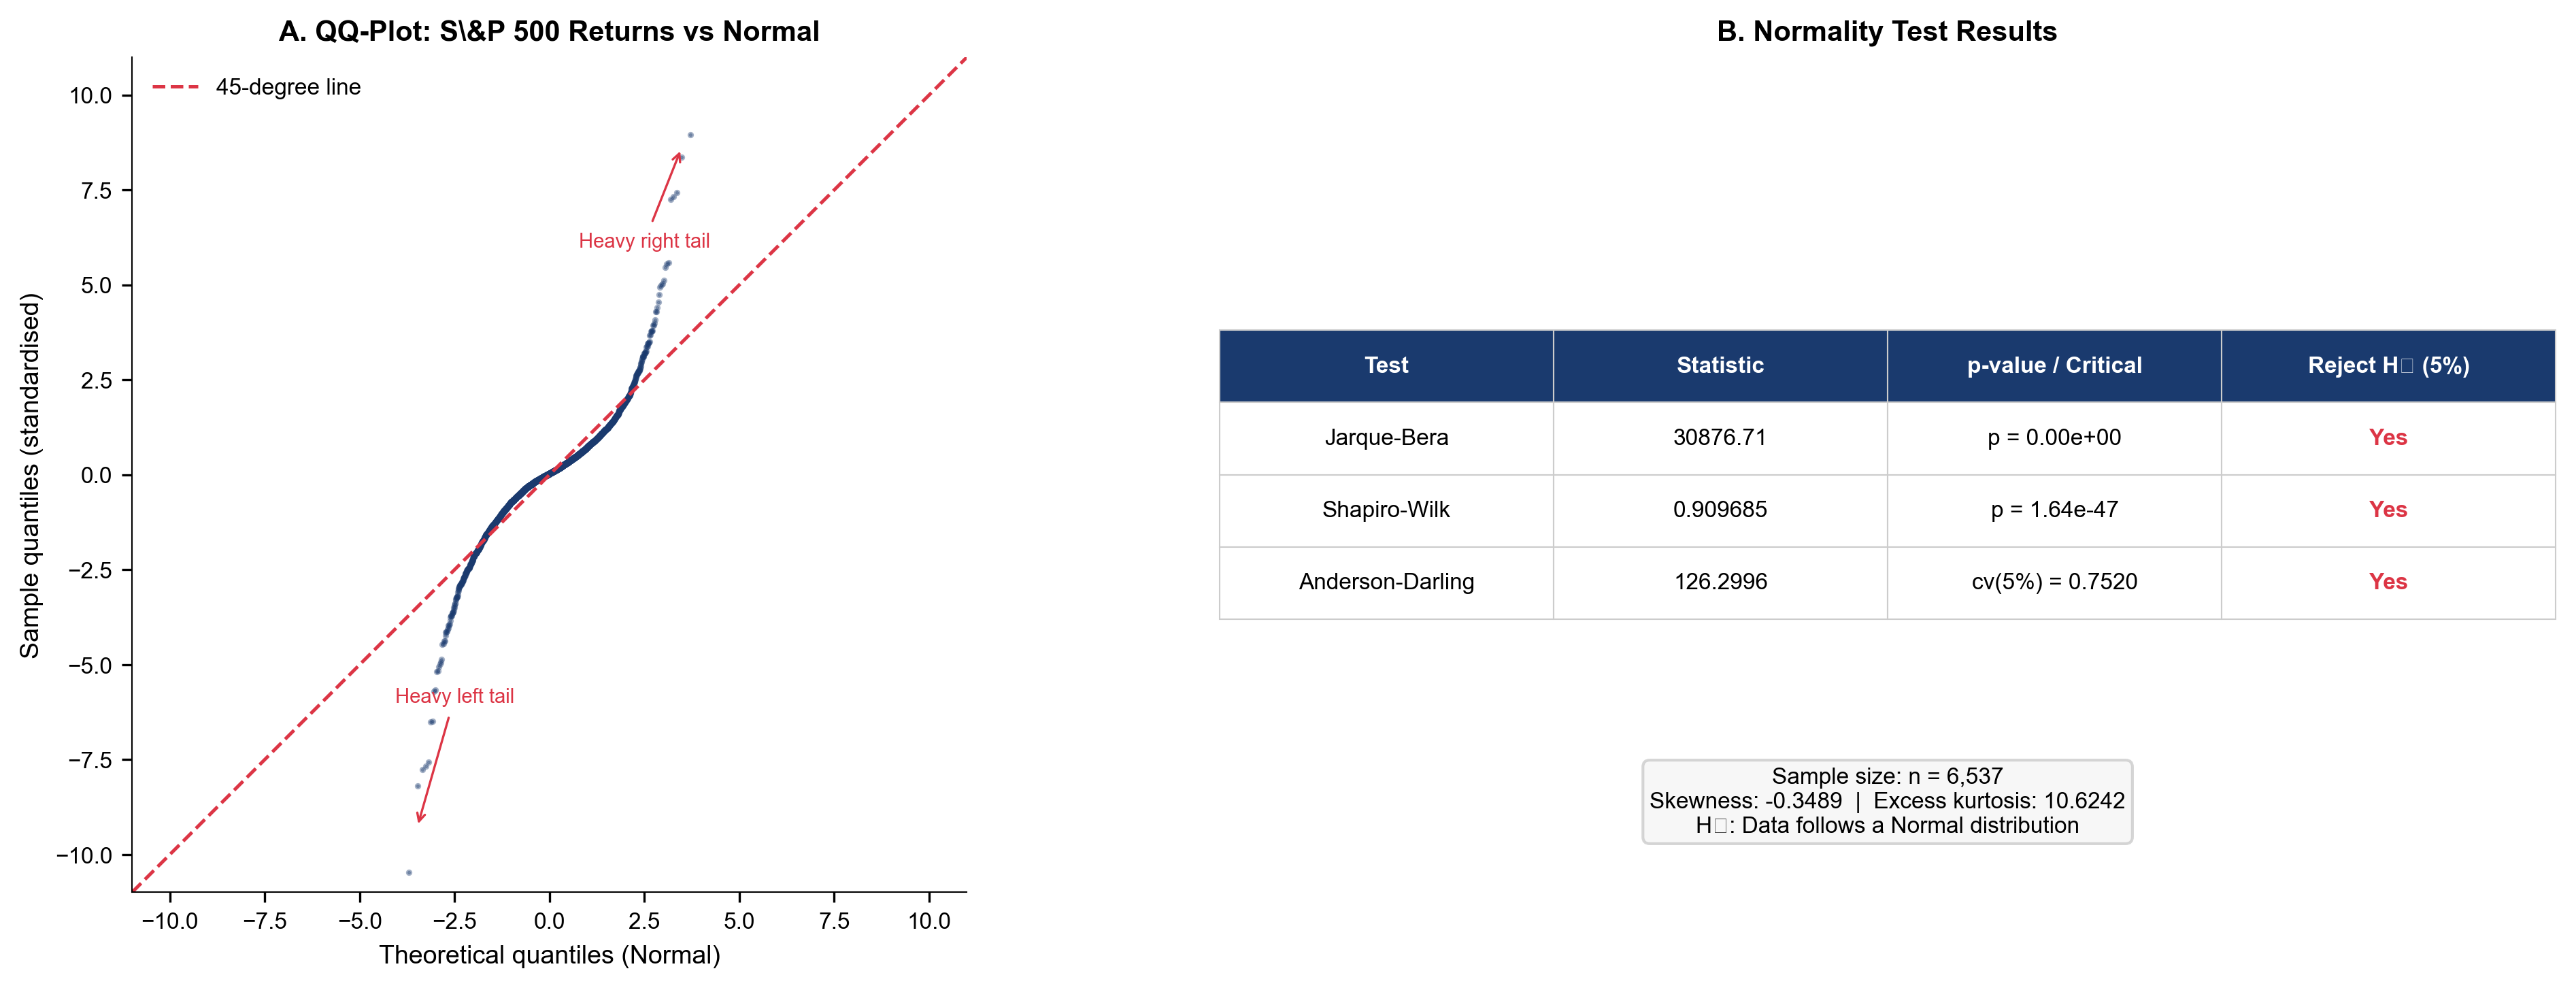
\includegraphics[width=0.68\textwidth]{ch2_normality_tests.png}
\end{center}
\quantlet{SFM\_ch2\_normal\_distribution}{https://github.com/QuantLet/Stat_fin_markets/tree/master/Ch_02/SFM_ch2_normal_distribution}
\begin{itemize}
\item Rezultatele testelor pe randamentele S\&P~500 resping \textbf{masiv} ipoteza de normalitate
\item Testul JB: $p$-value $\approx 0$ (asimetrie și kurtosis diferite de valorile normale)
\end{itemize}
\end{frame}

%--- MSc Slide 6 ---
\slidelevel{MSc}
\begin{frame}{Teste de normalitate --- Rezultate empirice (S\&P 500)}
\vspace{0.2cm}
\begin{center}
\renewcommand{\arraystretch}{1.5}
\large
\begin{tabular}{lccc}
\toprule
\textbf{Test} & \textbf{Statistica} & \textbf{$p$-value} & \textbf{Decizia} \\
\midrule
Jarque--Bera & $>1000$ & $<0{,}001$ & \textcolor{Crimson}{\textbf{Respingem} $H_0$} \\
Shapiro--Wilk & $<0{,}99$ & $<0{,}001$ & \textcolor{Crimson}{\textbf{Respingem} $H_0$} \\
Anderson--Darling & $>10$ & $<0{,}001$ & \textcolor{Crimson}{\textbf{Respingem} $H_0$} \\
Kolmogorov--Smirnov & $>0{,}05$ & $<0{,}001$ & \textcolor{Crimson}{\textbf{Respingem} $H_0$} \\
\bottomrule
\end{tabular}
\end{center}

\vspace{0.2cm}
\begin{alertblock}{Concluzie}
Normalitatea este respinsă \textbf{covârșitor} pentru randamentele financiare zilnice.
Distribuția normală subestimează sistematic riscul de coadă.
\end{alertblock}
\end{frame}

%--- PhD Slide 7 ---
\slidelevel{PhD}
\begin{frame}{Marginile Berry--Esseen și ratele de convergență}
\begin{thm}[Berry--Esseen]
Dacă $X_1, X_2, \ldots$ sunt i.i.d.\ cu $\E[X_i]=0$, $\E[X_i^2]=\sigma^2$, $\E[|X_i|^3]=\rho < \infty$, atunci:
\[
\sup_x \left|F_n(x) - \Phi(x)\right| \leq \frac{C\,\rho}{\sigma^3\sqrt{n}}
\]
unde $C \leq 0{,}4748$ (Shevtsova, 2011).
\end{thm}

\begin{itemize}
\item Rata de convergență: $O(n^{-1/2})$ --- lentă pentru date cu cozi groase
\item Expansiunile Edgeworth rafinează aproximarea TLC pentru $n$ finit
\item \textbf{Distribuția normală ca distribuție stabilă}: $N(\mu,\sigma^2) = S(2, 0, \sigma/\sqrt{2}, \mu)$ --- membrul $\alpha=2$ al familiei stabile
\item Când $\E[X_i^2] = \infty$: TLC eșuează, dar \textbf{TLC Generalizată} dă limite stabile
\end{itemize}
\end{frame}

%--- Y3 Slide 8 ---
\slidelevel{Y3}
\begin{frame}{Exemplu: Probabilitatea unei pierderi mari sub distribuția normală}
\begin{exampleblock}{Exercițiu}
Un portofoliu are $\sigma = 1{,}5\%$ zilnic. Sub ipoteza normală cu $\mu = 0$, calculați $P(\text{pierdere} > 3\sigma)$. Câte zile pe an se așteaptă o astfel de pierdere? Comparați cu frecvența empirică.
\end{exampleblock}

\begin{block}{Rezolvare}
$P(r < -3\sigma) = \Phi(-3) = 0{,}00135$ (0{,}135\%). Cu 252 zile/an: $252 \times 0{,}00135 = \mathbf{0{,}34}$ zile/an (o dată la $\sim$3 ani).
\end{block}

\begin{alertblock}{Realitatea empirică}
\begin{itemize}
\item S\&P~500 (1990--2023): pierderi $> 4{,}5\%$ apar $\approx 0{,}7$ ori/an --- \textbf{2$\times$ mai frecvent} decât sub distribuția normală
\item Pierderi $> 5\sigma$: distribuția normală prevede 1 eveniment la 13.932 ani; empiric, apare la decenii
\item \textbf{Concluzie}: Distribuția normală subestimează dramatic riscul de coadă
\end{itemize}
\end{alertblock}
\end{frame}

%=============================================================================
% SECȚIUNEA 4: FAPTE STILIZATE ALE RANDAMENTELOR FINANCIARE
%=============================================================================
\section{Fapte stilizate ale randamentelor financiare}

%--- Y3 Slide 1 ---
\slidelevel{Y3}
\begin{frame}{Cozi groase și exces de kurtosis}
\begin{itemize}
\item \textbf{Kurtosis}: $\kappa = \E[(X-\mu)^4]/\sigma^4$; \quad exces de kurtosis: $\kappa_e = \kappa - 3$
\item Distribuția normală: $\kappa_e = 0$
\item Kurtosis tipică pentru acțiuni zilnice: $\kappa \in [5, 50]$, deci $\kappa_e \gg 0$
\item \textbf{Interpretare}: Randamentele extreme apar mult mai frecvent decât prevede distribuția normală
\end{itemize}

\vspace{0.2cm}
\begin{center}
\renewcommand{\arraystretch}{1.1}
\begin{tabular}{lcc}
\toprule
\textbf{Activ} & \textbf{Asimetrie} & \textbf{Exces de kurtosis} \\
\midrule
S\&P 500 (zilnic) & $-0{,}3$ & $\approx 10$ \\
FTSE 100 (zilnic) & $-0{,}2$ & $\approx 8$ \\
USD/EUR (zilnic) & $-0{,}1$ & $\approx 5$ \\
Bitcoin (zilnic) & $-0{,}5$ & $\approx 15$ \\
\bottomrule
\end{tabular}
\end{center}
\end{frame}

%--- Y3 Slide 2 ---
\slidelevel{Y3}
\begin{frame}{Asimetrie negativă și clusterizarea volatilității}
\begin{columns}[T]
\begin{column}{0.48\textwidth}
\begin{block}{Asimetrie negativă}
\begin{itemize}
\item Coada stângă mai grea decât cea dreaptă
\item Mai pronunțată pentru indici de acțiuni
\item Prăbușirile sunt mai abrupte decât raliul
\item Asimetrie $S = \E[(X-\mu)^3]/\sigma^3 < 0$
\end{itemize}
\end{block}
\end{column}
\begin{column}{0.48\textwidth}
\begin{block}{Clusterizarea volatilității}
\begin{itemize}
\item ,,Variații mari urmate de variații mari'' (Mandelbrot, 1963)
\item $\Corr(|r_t|, |r_{t+k}|) > 0$ pentru $k$ mare
\item Randamentele sunt necorelate dar \textbf{nu independente}
\item $\Corr(r_t, r_{t+k}) \approx 0$ dar $\Corr(r_t^2, r_{t+k}^2) > 0$
\end{itemize}
\end{block}
\end{column}
\end{columns}

\vspace{0.3cm}
\begin{block}{Implicație}
\begin{itemize}
\item O singură distribuție i.i.d.\ nu poate surprinde clusterizarea volatilității
\item Avem nevoie de modele cu varianță variabilă în timp (GARCH, Secțiunea~2.10)
\end{itemize}
\end{block}
\end{frame}

%--- Y3 Slide 3 ---
\slidelevel{Y3}
\begin{frame}{Gaussianitate agregată}
\begin{itemize}
\item \textbf{Observație cheie}: Pe măsură ce orizontul de deținere crește, distribuția randamentelor devine \textit{mai Gaussiană}
\item Randamente zilnice: kurtosis ridicată, cozi groase
\item Randamente săptămânale: kurtosis moderată
\item Randamente lunare: mai aproape de distribuția normală
\item \textbf{Mecanism}: Efect similar TLC --- randamentul lunar $= \sum$ din $\sim$22 randamente zilnice
\end{itemize}

\vspace{0.2cm}
\begin{center}
\renewcommand{\arraystretch}{1.1}
\begin{tabular}{lcc}
\toprule
\textbf{Frecvență} & \textbf{Exces de kurtosis} & \textbf{JB $p$-value} \\
\midrule
Zilnică & $\approx 10$ & $< 0{,}001$ \\
Săptămânală & $\approx 4$ & $< 0{,}001$ \\
Lunară & $\approx 1{,}5$ & $\approx 0{,}05$ \\
Trimestrială & $\approx 0{,}5$ & $\approx 0{,}3$ \\
\bottomrule
\end{tabular}
\end{center}
\end{frame}

%--- Y3 Slide 4 ---
\slidelevel{Y3}
\begin{frame}{Rezumatul faptelor stilizate}
\begin{enumerate}
\item \textbf{Cozi groase}: $\kappa_e \gg 0$ --- evenimente extreme mai frecvente decât sub normală
\item \textbf{Asimetrie negativă}: Coada stângă mai grea (acțiuni)
\item \textbf{Clusterizarea volatilității}: Perioade de volatilitate mare/mică persistă
\item \textbf{Gaussianitate agregată}: Kurtosis scade cu orizontul
\item \textbf{Absența autocorelației randamentelor}: $\Corr(r_t, r_{t+k}) \approx 0$ pentru $k \geq 1$
\item \textbf{Autocorelația randamentelor pătrate}: $\Corr(r_t^2, r_{t+k}^2) > 0$
\end{enumerate}

\vspace{0.3cm}
\begin{alertblock}{Provocarea}
\begin{itemize}
\item Orice model adecvat pentru randamentele financiare trebuie să reproducă aceste fapte stilizate
\item Distribuția normală eșuează la punctele 1, 2 și 3
\end{itemize}
\end{alertblock}
\end{frame}

%--- MSc Slide 5 ---
\slidelevel{MSc}
\begin{frame}{Efectul de levier și memoria lungă}
\begin{columns}[T]
\begin{column}{0.48\textwidth}
\begin{block}{Efectul de levier}
\begin{itemize}
\item Randamentele negative cresc volatilitatea viitoare \textit{mai mult} decât randamentele pozitive de aceeași magnitudine
\item Răspuns asimetric: $\Corr(r_t, \sigma_{t+1}^2) < 0$
\item Denumit după Black (1976): scăderea prețului $\Rightarrow$ levier mai mare $\Rightarrow$ risc mai mare
\item Capturat de GJR-GARCH, EGARCH
\end{itemize}
\end{block}
\end{column}
\begin{column}{0.48\textwidth}
\begin{block}{Memoria lungă în volatilitate}
\begin{itemize}
\item $\Corr(|r_t|, |r_{t+k}|)$ scade \textit{lent} (hiperbolic, nu exponențial)
\item Exponentul Hurst $H > 0{,}5$ pentru $|r_t|$
\item GARCH standard: descreștere exponențială
\item Modelele FIGARCH, HAR surprind memoria lungă
\end{itemize}
\end{block}
\end{column}
\end{columns}
\end{frame}

%--- MSc Slide 6 ---
\slidelevel{MSc}
\begin{frame}{Asimetria câștig/pierdere}
\begin{itemize}
\item \textbf{Asimetria câștig/pierdere}: Prețurile acțiunilor scad mai repede decât cresc
\item Scăderile mari au loc în zile; recuperarea durează luni sau ani
\item Această asimetrie este distinctă de asimetria distribuției --- privește \textit{dinamica}, nu distribuția marginală
\item \textbf{Efect volumetric}: Volumul de tranzacționare crește în episoadele de volatilitate mare
\begin{itemize}
\item Corelație pozitivă între $|r_t|$ și volumul zilnic
\item Amplificată de \textit{margin calls} și vânzări forțate
\end{itemize}
\end{itemize}
\end{frame}

%--- PhD Slide 7 ---
\slidelevel{PhD}
\begin{frame}{Taxonomia Cont (2001) și modele multifractale}
\begin{itemize}
\item Cont (2001): taxonomie sistematică a 11 fapte stilizate pentru randamentele activelor
\item \textbf{Modele multifractale} (Mandelbrot, Fisher \& Calvet, 1997):
\begin{itemize}
\item $\E[|r_t|^q] \propto \Delta t^{\zeta(q)}$ cu $\zeta(q)$ \textit{neliniar} (multiscaling)
\item Unifractal: $\zeta(q) = qH$ (liniar); multifractal: $\zeta(q)$ concav
\end{itemize}
\item Structura corelațiilor încrucișate și fapte stilizate multivariate
\item Fapte stilizate intra-zilnice: zgomot de microstructură, săritura bid-ask, efectul Epps
\end{itemize}
\end{frame}

%--- PhD Slide 8 ---
\slidelevel{PhD}
\begin{frame}{Structura fractală și legile putere}
\begin{itemize}
\item \textbf{Cozi tip lege putere (\textit{power law})}: $P(|r| > x) \sim x^{-\alpha}$ cu $\alpha \in [2, 5]$ pentru majoritatea activelor financiare
\item Exponentul de coadă $\alpha$ este remarcabil de stabil între active și perioade
\item \textbf{Auto-similaritate}: Distribuțiile randamentelor la scale temporale diferite sunt legate prin scalare
\item Conexiunea cu distribuțiile stabile: dacă $\alpha < 2$, TLC Generalizată implică limite stabile
\item ,,Legea cubului invers'' (Gopikrishnan et al., 1999): $\alpha \approx 3$ pentru acțiunile americane
\item Dezbatere: lege putere reală vs.\ cozi cu variație lentă
\end{itemize}
\end{frame}

%--- Y3 Slide 9 ---
\slidelevel{Y3}
\begin{frame}{Vizualizarea clusterizării volatilității}
\vspace{-0.2cm}
\begin{center}
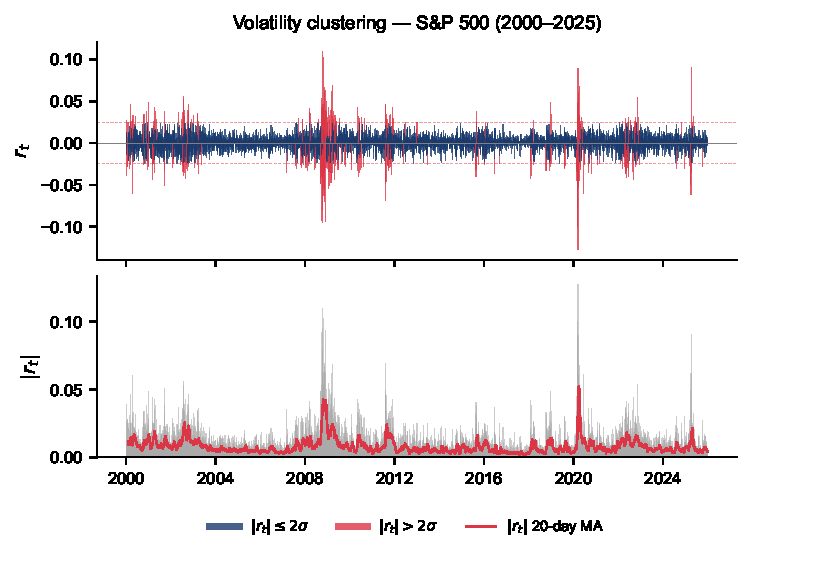
\includegraphics[width=0.50\linewidth]{ch2_volatility_clustering.pdf}
\end{center}
\vspace{-0.4cm}
\quantlet{SFM\_ch2\_stylized\_facts}{https://github.com/QuantLet/Stat_fin_markets/tree/master/Ch_02/SFM_ch2_stylized_facts}
\begin{itemize}\setlength\itemsep{0pt}
\item ,,Variații mari urmate de variații mari'' (Mandelbrot, 1963) --- crizele 2001, 2008, 2020
\item $\Corr(r_t, r_{t+k}) \approx 0$ dar $\Corr(|r_t|, |r_{t+k}|) > 0$ --- necorelate, dar \textbf{nu independente}
\end{itemize}
\end{frame}

%--- Y3 Slide 10 ---
\slidelevel{Y3}
\begin{frame}{Ecuațiile faptelor stilizate --- Kurtosis și autocorelația}
\begin{columns}[T]
\begin{column}{0.48\textwidth}
\begin{block}{Kurtosis}
\[
\kappa = \frac{\E[(X - \mu)^4]}{\sigma^4}
\]
\begin{itemize}
\item \textbf{Exces de kurtosis}: $\kappa_e = \kappa - 3$
\item $\kappa_e = 0$: distribuția normală (referință)
\item $\kappa_e > 0$: \textbf{leptocurtică} (cozi groase --- \textit{fat tails})
\end{itemize}
\end{block}
\begin{block}{Autocorelația $r_t^2$}
\[
\rho_k = \Corr(r_t^2, r_{t+k}^2) > 0, \quad k \text{ mare}
\]
\end{block}
\end{column}
\begin{column}{0.48\textwidth}
\begin{exampleblock}{Exemplu numeric}
\renewcommand{\arraystretch}{1.1}
\begin{tabular}{lcc}
\toprule
& $\kappa$ & $\kappa_e$ \\
\midrule
Normal & 3 & 0 \\
S\&P 500 & $\approx$10 & $\approx$7 \\
FTSE 100 & $\approx$8 & $\approx$5 \\
Bitcoin & $\approx$15 & $\approx$12 \\
\bottomrule
\end{tabular}
\end{exampleblock}

\vspace{0.1cm}
{\small $\kappa_e = 7$ pentru S\&P~500 $\Rightarrow$ cozi \textbf{substanțial mai groase} decât distribuția normală}
\end{column}
\end{columns}
\end{frame}

%--- Y3 Slide 11: Previzualizare VaR/ES (necesar pentru Secțiunile 5-8) ---
\slidelevel{Y3}
\begin{frame}{Previzualizare: Măsuri de risc --- VaR și ES}
\begin{defn}[Value-at-Risk --- definiție de lucru]
\textbf{Value-at-Risk} la nivelul $\alpha$: pierderea maximă care \textbf{nu} este depășită cu probabilitatea $(1-\alpha)$:
\[
\text{VaR}_\alpha = -F^{-1}(\alpha), \quad \text{unde } F^{-1} \text{ este cuantila randamentelor.}
\]
\end{defn}
\vspace{-0.15cm}
\begin{defn}[Expected Shortfall --- definiție de lucru]
\textbf{Expected Shortfall} (ES) la nivelul $\alpha$: pierderea \textbf{medie} în cele mai rele $\alpha\%$ scenarii:
\[
\text{ES}_\alpha = -\frac{1}{\alpha}\int_0^\alpha F^{-1}(p)\,dp.
\]
\end{defn}
\vspace{-0.15cm}
\begin{itemize}
\item \textbf{Exemplu}: VaR 1\% normală, $\sigma = 1{,}5\%$, \$1M: $\text{VaR} = 2{,}326 \times 0{,}015 \times 10^6 = \$34.890$
\item Proprietăți formale, coerența Artzner, backtesting --- \textbf{Secțiunea 10}
\end{itemize}
\end{frame}

%--- Y3 Slide 12: Ilustrare grafică VaR/ES ---
\slidelevel{Y3}
\begin{frame}{VaR și ES --- Ilustrare grafică}
\begin{center}
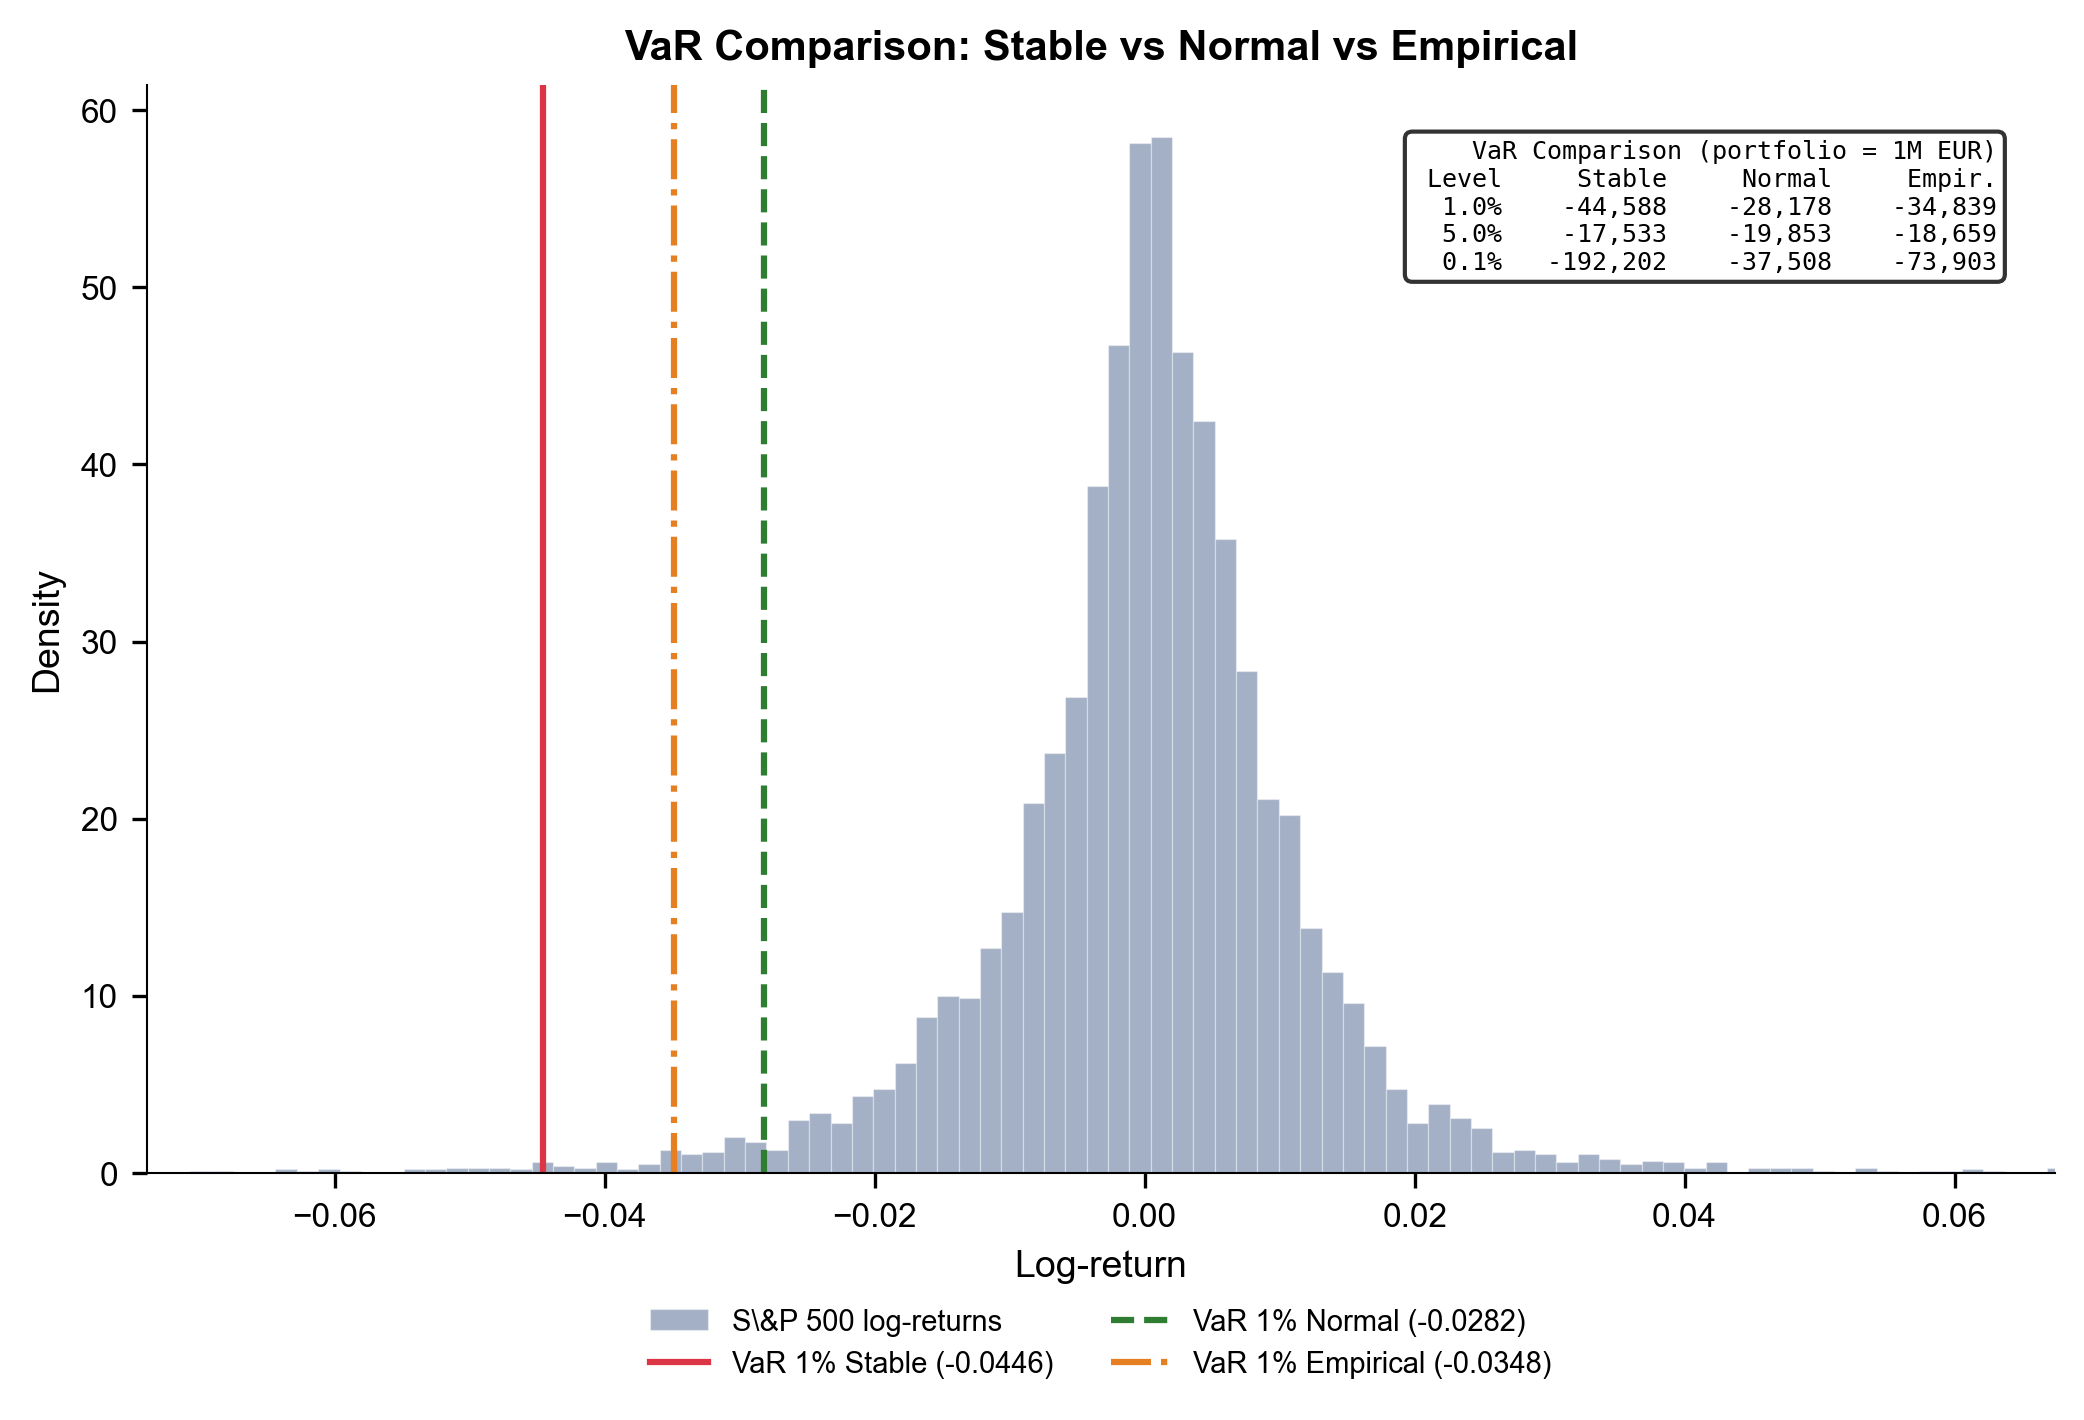
\includegraphics[width=0.48\textwidth]{ch2_var_comparison.png}
\end{center}
\vspace{-0.3cm}
\quantlet{SFM\_ch2\_risk\_management}{https://github.com/QuantLet/Stat_fin_markets/tree/master/Ch_02/SFM_ch2_risk_management}
\vspace{-0.15cm}
\begin{itemize}\setlength{\itemsep}{1pt}
\item \textbf{VaR}$_\alpha$: cuantila --- „nu vom pierde mai mult de $X$ cu prob.\ $1-\alpha$"
\item \textbf{ES}$_\alpha$: media cozii --- „dacă depășim VaR, cât pierdem \textit{în medie}?"
\item ES $\geq$ VaR întotdeauna; diferența crește cu grosimea cozilor
\end{itemize}
\end{frame}

%=============================================================================
% TITLU PARTEA II

%=============================================================================
% TITLU PARTEA II
%=============================================================================
% SECȚIUNEA 5: DISTRIBUȚIA STUDENT-T
%=============================================================================
\section{Distribuția Student-$t$}

%--- Y3 Slide 1 ---
\slidelevel{Y3}
\begin{frame}{Distribuția Student-$t$ --- Definiție}
\begin{defn}[Distribuția Student-$t$]
$X \sim t_\nu$ dacă:
\[
f(x;\nu) = \frac{\Gamma\!\left(\frac{\nu+1}{2}\right)}{\sqrt{\nu\pi}\,\Gamma\!\left(\frac{\nu}{2}\right)} \left(1 + \frac{x^2}{\nu}\right)^{-(\nu+1)/2}, \quad x \in \R.
\]
\end{defn}

\begin{itemize}
\item Un singur parametru $\nu > 0$ (\textbf{grade de libertate}) controlează grosimea cozilor
\item $\E[X] = 0$ ($\nu > 1$); \quad $\Var(X) = \frac{\nu}{\nu-2}$ ($\nu > 2$)
\item Exces de kurtosis: $\kappa_e = \frac{6}{\nu-4}$ ($\nu > 4$)
\item $\nu \to \infty$: converge la $N(0,1)$; \quad $\nu = 1$: distribuția Cauchy
\item Cozi: $f(x) \sim |x|^{-(\nu+1)}$ \textbf{(lege putere)}
\end{itemize}
\end{frame}

%--- Y3 Slide 2 ---
\slidelevel{Y3}
\begin{frame}{PDF-uri Student-$t$ --- Efectul lui $\nu$}
\begin{center}
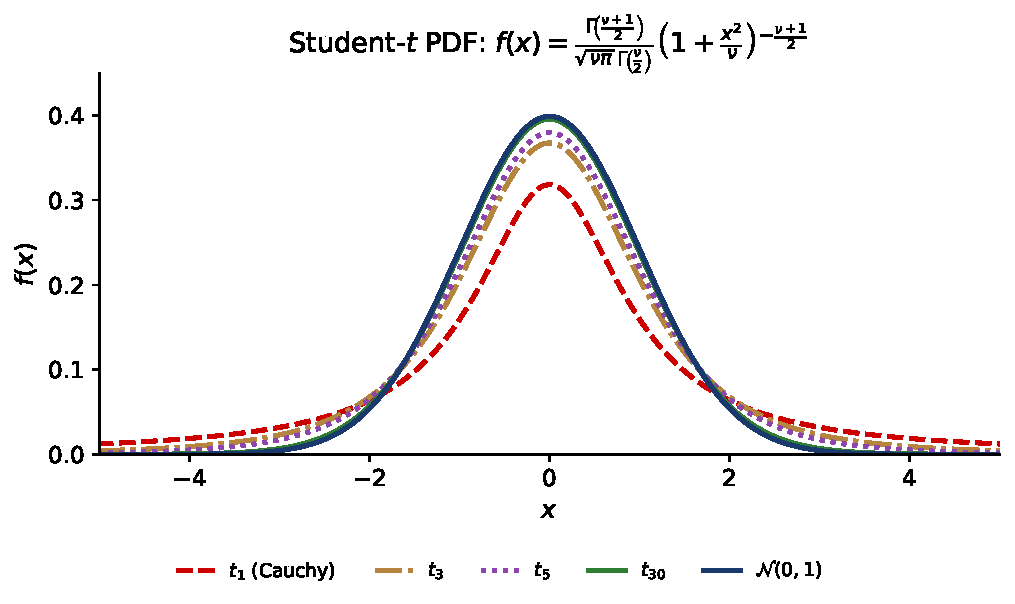
\includegraphics[width=0.58\textwidth]{ch2_student_t_pdf_theoretical.pdf}
\end{center}
\quantlet{SFM\_ch2\_student\_t}{https://github.com/QuantLet/Stat_fin_markets/tree/master/Ch_02/SFM_ch2_student_t}

\begin{itemize}
\item $\nu$ mai mic $\Rightarrow$ cozi mai groase, vârf mai ascuțit
\item Randamente financiare: de regulă $\hat{\nu} \in [3, 8]$ pentru date zilnice de acțiuni
\end{itemize}
\end{frame}

%--- Y3 Slide 3 ---
\slidelevel{Y3}
\begin{frame}{Ajustarea Student-$t$ pe S\&P 500}
\begin{center}
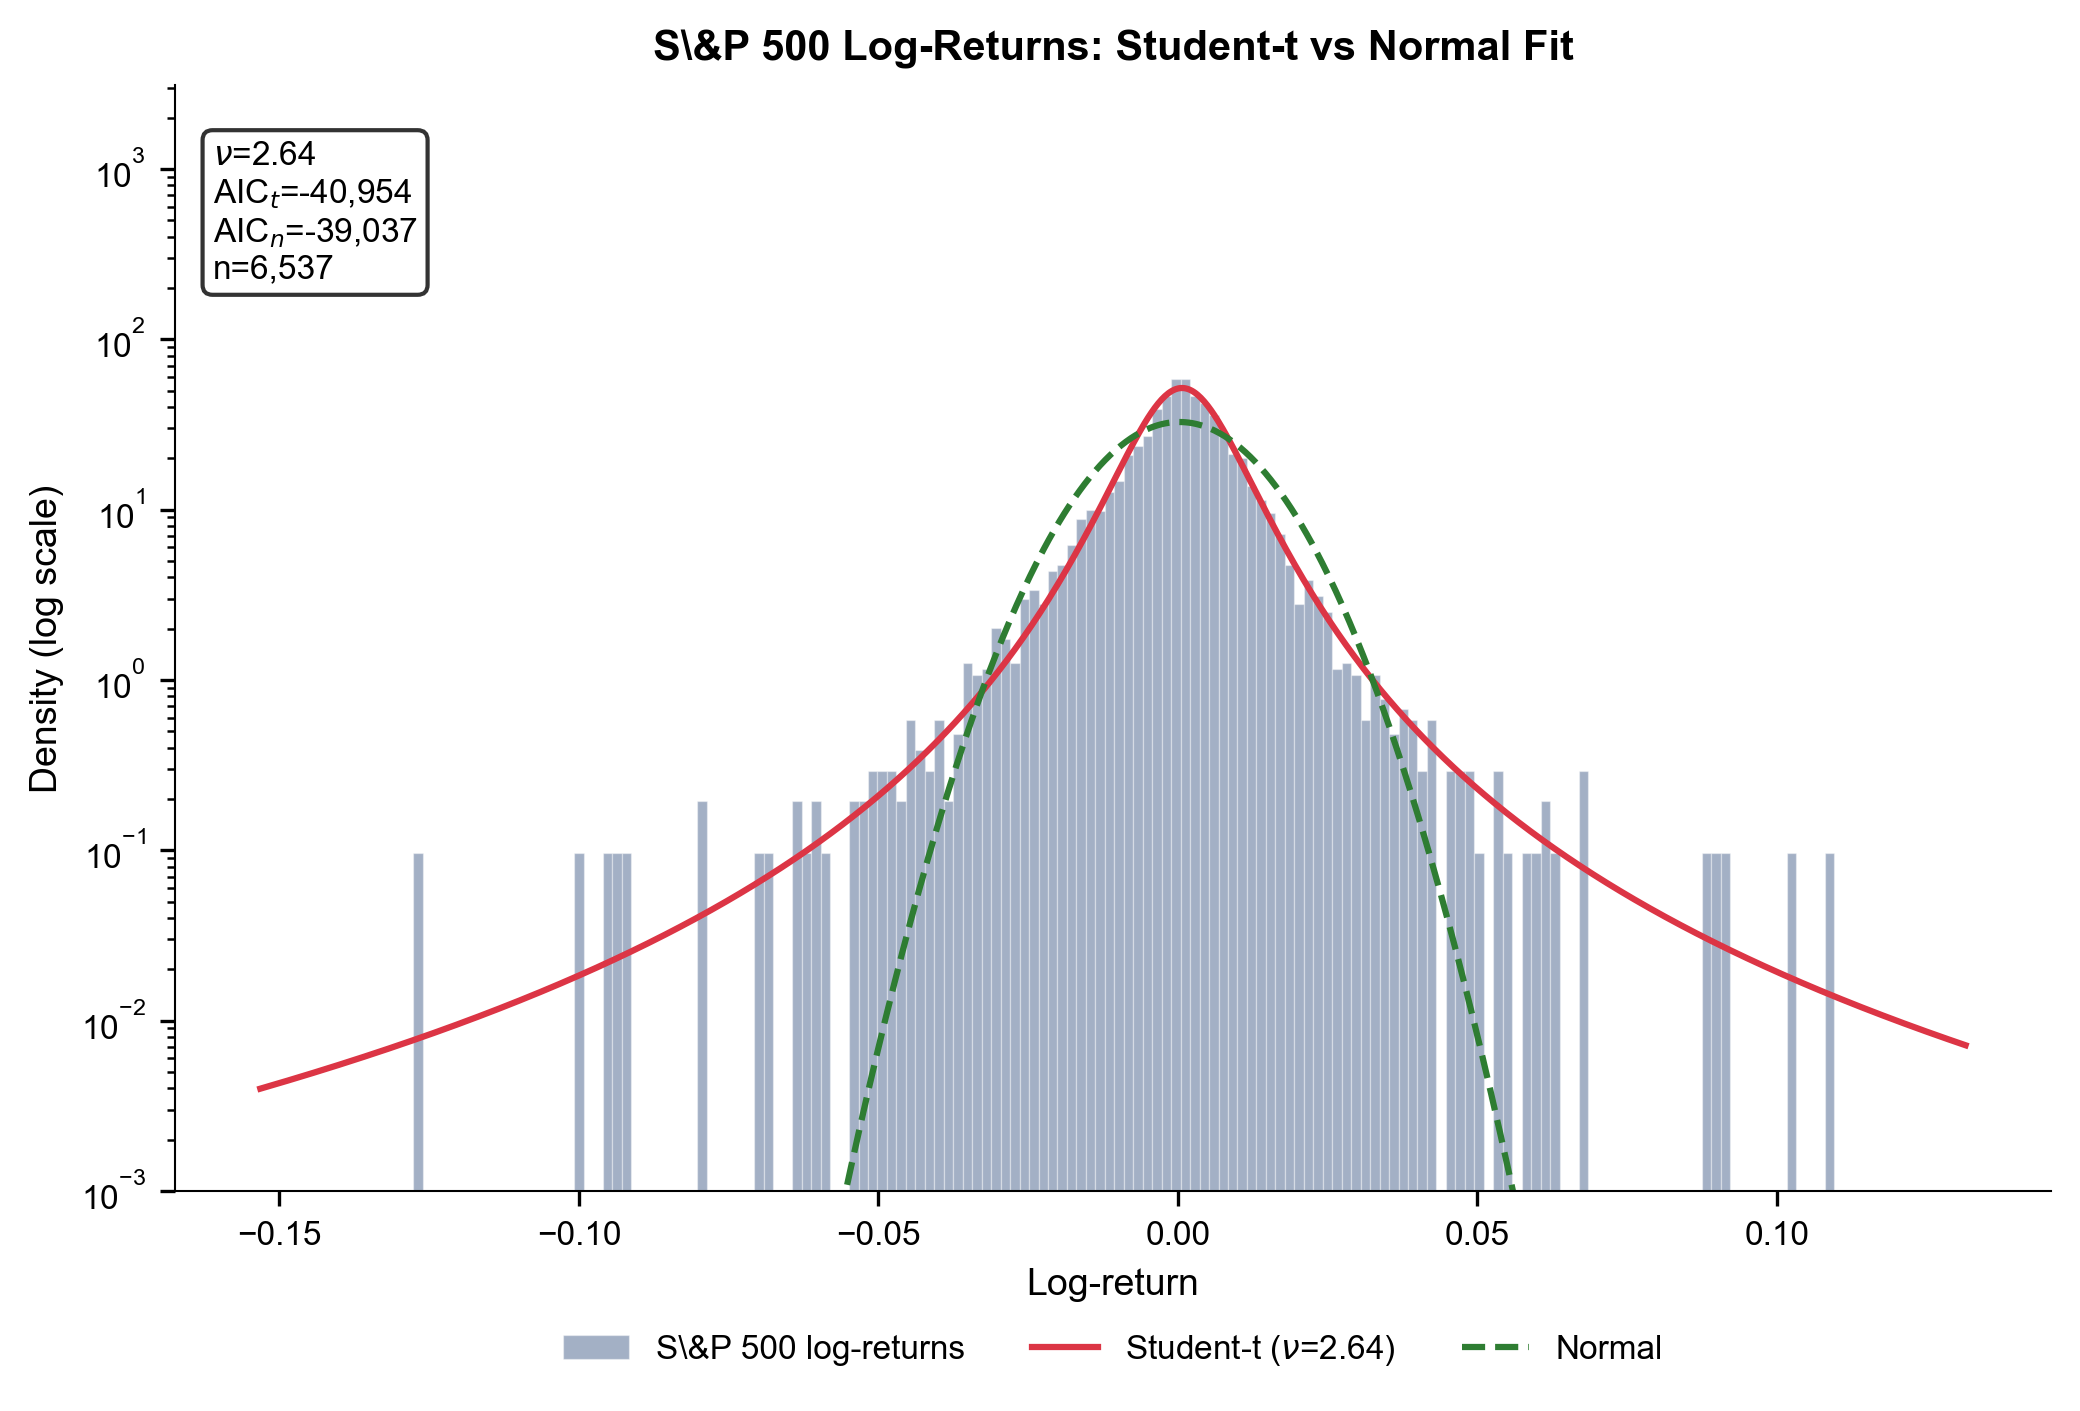
\includegraphics[width=0.45\textwidth]{ch2_student_t_fit.png}
\end{center}
\quantlet{SFM\_ch2\_student\_t}{https://github.com/QuantLet/Stat_fin_markets/tree/master/Ch_02/SFM_ch2_student_t}
\begin{itemize}
\item Student-$t$ surprinde cozile groase mult mai bine decât distribuția normală
\item $\hat{\nu} \approx 4$--$5$ pentru S\&P~500; centrul și cozile bine ajustate
\end{itemize}
\end{frame}

%--- Y3 Slide 4 ---
\slidelevel{Y3}
\begin{frame}{De ce Student-$t$ pentru finanțe?}
\begin{center}
\renewcommand{\arraystretch}{1.2}
\begin{tabular}{lcc}
\toprule
\textbf{Proprietate} & \textbf{Normal} & \textbf{Student-$t$} \\
\midrule
Descreșterea cozii & Exponențială ($e^{-x^2/2}$) & Lege putere ($|x|^{-\nu-1}$) \\
Exces de kurtosis & 0 & $6/(\nu-4)$ \\
Parametri & 2 ($\mu, \sigma$) & 3 ($\mu, \sigma, \nu$) \\
Evenimente extreme & Foarte rare & Mai frecvente \\
Limită & --- & Normal ($\nu \to \infty$) \\
\bottomrule
\end{tabular}
\end{center}

\vspace{0.3cm}
\begin{block}{Avantaj cheie}
\begin{itemize}
\item Student-$t$ \textbf{include} distribuția normală ca un caz special ($\nu \to \infty$) permițând în același timp cozi mai groase
\item Este cea mai simplă alternativă cu cozi groase
\end{itemize}
\end{block}
\end{frame}

%--- MSc Slide 5 ---
\slidelevel{MSc}
\begin{frame}{Forma locație-scală și MLE}
\begin{itemize}
\item \textbf{Forma locație-scală}: $X = \mu + \sigma T$, unde $T \sim t_\nu$
\item Estimare MLE a $(\mu, \sigma, \nu)$: maximizăm
\[
\ell(\mu,\sigma,\nu) = \sum_{t=1}^{n} \ln f\!\left(\frac{r_t - \mu}{\sigma}; \nu\right) - n\ln\sigma
\]
\item Criterii informaționale pentru selecția modelului:
\begin{itemize}
\item AIC $= -2\ell + 2k$ (penalizează ușor complexitatea)
\item BIC $= -2\ell + k\ln n$ (penalizează mai puternic complexitatea)
\end{itemize}
\item Student-$t$ ca distribuție a inovațiilor în modele GARCH: $\epsilon_t = \sigma_t z_t$, $z_t \sim t_\nu$
\item Diagnostice QQ-plot: abaterile de la linia de 45$^\circ$ indică specificare greșită
\end{itemize}
\end{frame}

%--- MSc Slide 6 ---
\slidelevel{MSc}
\begin{frame}{Compararea modelelor: normală vs.\ Student-$t$}
\begin{center}
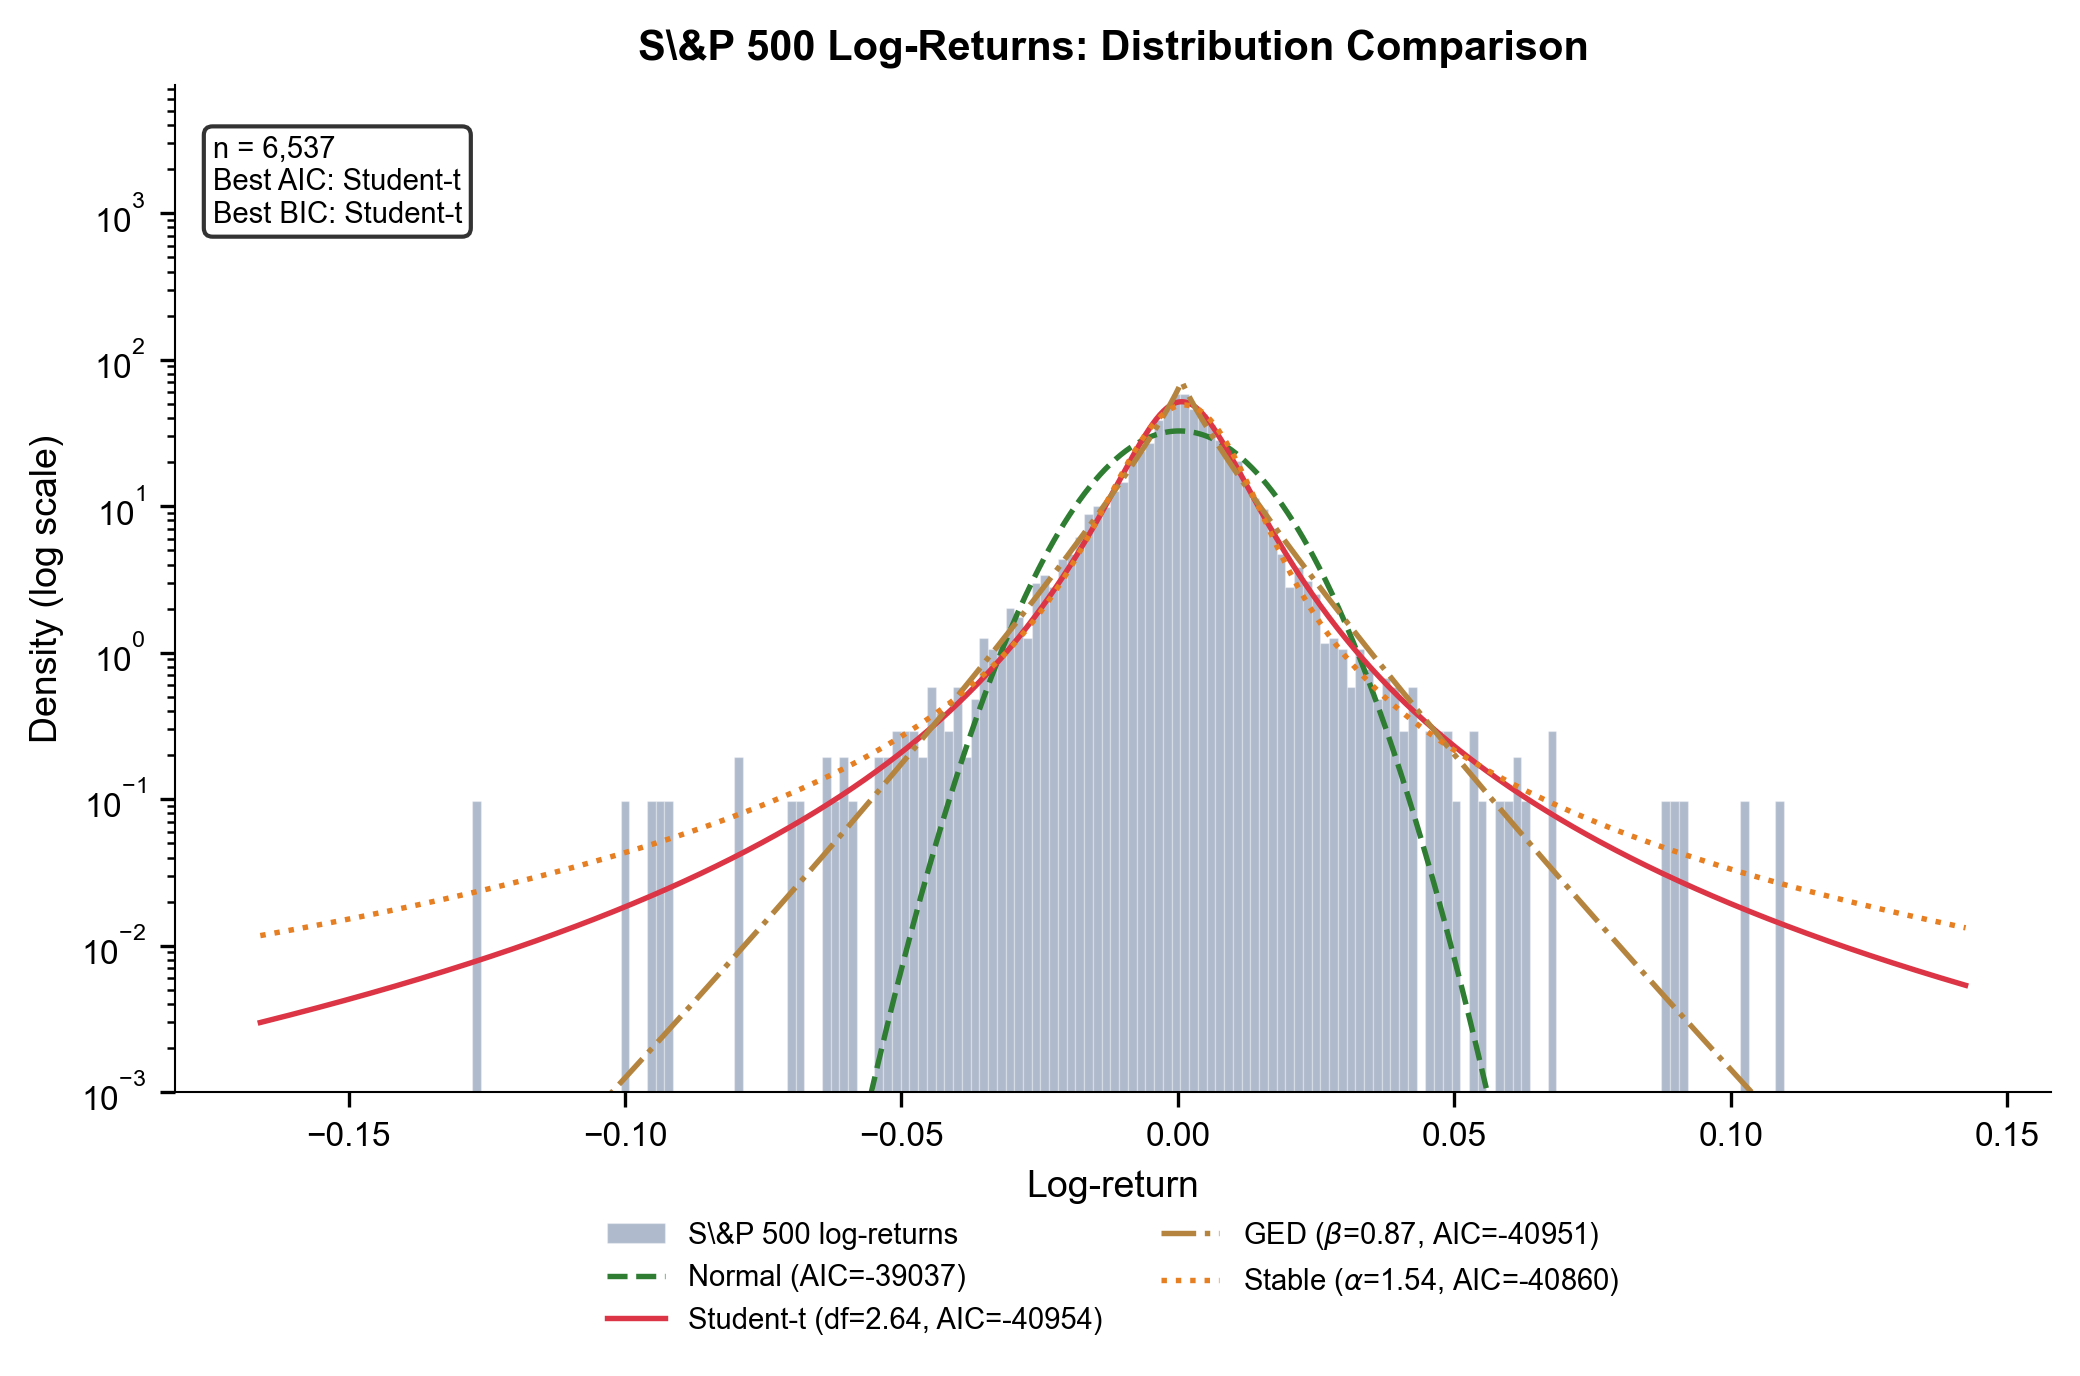
\includegraphics[width=0.38\textwidth]{ch2_dist_comparison_overlay.png}
\end{center}
\quantlet{SFM\_ch2\_distribution\_comparison}{https://github.com/QuantLet/Stat_fin_markets/tree/master/Ch_02/SFM_ch2_distribution_comparison}
\begin{center}
\renewcommand{\arraystretch}{1.0}
\footnotesize
\begin{tabular}{lccc}
\toprule
\textbf{Model} & \textbf{Log-verosim.} & \textbf{AIC} & \textbf{BIC} \\
\midrule
Normal $(\mu, \sigma)$ & $\ell_1$ & $-2\ell_1 + 4$ & $-2\ell_1 + 2\ln n$ \\
Student-$t$ $(\mu, \sigma, \nu)$ & $\ell_2 > \ell_1$ & $-2\ell_2 + 6$ & $-2\ell_2 + 3\ln n$ \\
\bottomrule
\end{tabular}
\end{center}
\begin{itemize}
\item Student-$t$ obține AIC/BIC substanțial mai bun în ciuda unui parametru suplimentar
\end{itemize}
\end{frame}

%--- PhD Slide 7 ---
\slidelevel{PhD}
\begin{frame}{Reprezentarea ca mixtură și interpretarea Bayesiană}
\begin{itemize}
\item \textbf{Reprezentare ca mixtură}: $X \mid V \sim N(0, V)$, \quad $V \sim \text{Inv-Gamma}(\nu/2, \nu/2)$
\begin{itemize}
\item Student-$t$ = Normală cu varianță aleatoare (mixtură de scale a normalelor)
\item Interpretare: $V$ surprinde volatilitatea variabilă în timp
\end{itemize}
\item \textbf{Interpretare Bayesiană}: Student-$t$ ca distribuție marginală a posteriori sub priori conjugate normal--inverse-gamma
\item \textbf{Student-$t$ multivariată}: $f(\bm{x}) \propto \left(1 + \frac{(\bm{x}-\bm{\mu})'\bm{\Sigma}^{-1}(\bm{x}-\bm{\mu})}{\nu}\right)^{-(\nu+p)/2}$
\item \textbf{Compararea cozilor}: indicele de coadă (\textit{tail index}) $t_\nu$ $= \nu$ vs.\ indicele de stabilitate $= \alpha$
\item Student-$t$ \textbf{nu} este închisă la convoluție; distribuțiile stabile \textbf{sunt}
\end{itemize}
\end{frame}

%--- Y3 Slide 8 ---
\slidelevel{Y3}
\begin{frame}{Exemplu: Probabilitatea unei pierderi extreme}
\begin{exampleblock}{Exercițiu}
Randamentele zilnice au $\sigma = 1{,}5\%$. Calculați $P(r < -3\sigma) = P(r < -4{,}5\%)$ sub distribuția normală vs.\ Student-$t$ cu $\nu = 5$.
\end{exampleblock}

\begin{block}{Rezolvare}
\begin{itemize}
\item \textbf{Sub distribuția normală}: $P(r < -3\sigma) = \Phi(-3) = 0{,}00135 = \mathbf{0{,}135\%}$ \quad (1 zi din 741)
\item \textbf{Sub Student-$t$ ($\nu = 5$)}: scală ajustată $s = \sigma\sqrt{(\nu-2)/\nu} = 0{,}01162$
\begin{itemize}
\item $t_{\text{stat}} = -0{,}045/0{,}01162 = -3{,}874 \;\Rightarrow\; P(T_5 < -3{,}874) = 0{,}00584 = \mathbf{0{,}584\%}$ \quad (1 zi din 171)
\end{itemize}
\end{itemize}
\end{block}

\begin{alertblock}{Concluzie}
\begin{itemize}
\item Student-$t$ prevede pierderi $> 3\sigma$ de \textbf{4{,}3$\times$ mai frecvent} decât distribuția normală ($0{,}584\%$ vs.\ $0{,}135\%$)
\end{itemize}
\end{alertblock}
\end{frame}

%=============================================================================
% SECȚIUNEA 5b: DISTRIBUȚIA PARETO
%=============================================================================
\section{Distribuția Pareto}

%--- Y3 Slide P1 ---
\slidelevel{Y3}
\begin{frame}{Distribuția Pareto --- Legea de putere}
\begin{block}{Definiție (Pareto, 1896)}
O variabilă aleatoare $X$ urmează o \textbf{distribuție Pareto} cu parametri $x_m > 0$ (scală) și $\alpha > 0$ (formă / indice de coadă) dacă:
\[
\boxed{\;f(x) = \frac{\alpha\, x_m^\alpha}{x^{\alpha+1}}, \quad x \geq x_m\;}
\]
\end{block}

\begin{columns}[T]
\begin{column}{0.48\textwidth}
\begin{itemize}\setlength\itemsep{2pt}
\item \textbf{CDF}: $F(x) = 1 - \left(\frac{x_m}{x}\right)^\alpha$
\item \textbf{Funcția de supraviețuire}:
\[
\bar{F}(x) = P(X > x) = \left(\frac{x_m}{x}\right)^\alpha
\]
\item Comportament \textbf{lege de putere} (\textit{power law}): $P(X > x) \propto x^{-\alpha}$
\end{itemize}
\end{column}
\begin{column}{0.48\textwidth}
\begin{itemize}\setlength\itemsep{2pt}
\item \textbf{Medie}: $\E[X] = \frac{\alpha\, x_m}{\alpha - 1}$ \quad (există doar dacă $\alpha > 1$)
\item \textbf{Varianță}: $\Var(X) = \frac{\alpha\, x_m^2}{(\alpha-1)^2(\alpha-2)}$ \quad (există doar dacă $\alpha > 2$)
\item $\alpha \leq 2$: \textbf{varianță infinită}
\item $\alpha \leq 1$: \textbf{medie infinită}
\end{itemize}
\end{column}
\end{columns}
\end{frame}

%--- Y3 Slide P1b: Graficul distribuției Pareto ---
\slidelevel{Y3}
\begin{frame}{Distribuția Pareto --- Grafic PDF și CDF}
\begin{center}
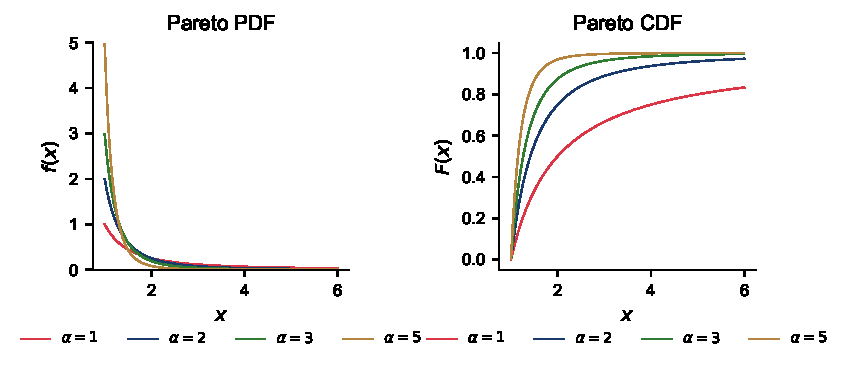
\includegraphics[width=0.78\textwidth]{ch2_pareto_pdf_cdf.pdf}
\end{center}
\vspace{-0.3cm}
\quantlet{SFM\_ch2\_pareto\_analysis}{https://github.com/QuantLet/Stat_fin_markets/tree/master/SFM_ch2/SFM_ch2_pareto_analysis}
\begin{itemize}\setlength\itemsep{2pt}
\item $\alpha$ mic $\Rightarrow$ coadă groasă, densitate scade lent
\item $\alpha$ mare $\Rightarrow$ masa se concentrează lângă $x_m$, coada scade rapid
\item CDF crește mai lent decât la distribuția normală --- probabilitate semnificativă în coadă
\end{itemize}
\end{frame}

%--- Y3 Slide P1c: Log-log survival (semnătura legii de putere) ---
\slidelevel{Y3}
\begin{frame}{Distribuția Pareto --- Semnătura legii de putere}
\begin{columns}[T]
\begin{column}{0.45\textwidth}
\vspace{-0.2cm}
\begin{center}
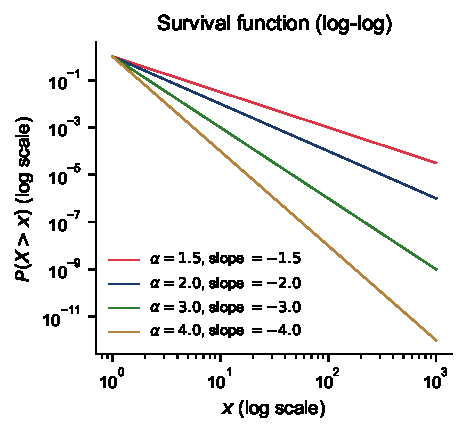
\includegraphics[width=\textwidth]{ch2_pareto_loglog_survival.pdf}
\end{center}
\end{column}
\begin{column}{0.52\textwidth}
\begin{block}{Testul grafic log-log}
\begin{itemize}\setlength\itemsep{2pt}
\item Pe graficul log-log, funcția de supraviețuire Pareto este o \textbf{dreaptă}:
\[
\log P(X > x) = -\alpha \log x + \alpha \log x_m
\]
\item \textbf{Panta} = $-\alpha$ (indicele de coadă)
\item Dacă datele empirice se aliniază pe o dreaptă $\Rightarrow$ comportament Pareto/lege de putere
\item Abaterea de la liniaritatePentru$x$ mici: \textit{trunchiere} sau alt mecanism de generare
\end{itemize}
\end{block}
\end{column}
\end{columns}
\end{frame}

%--- Y3 Slide P2 ---
\slidelevel{Y3}
\begin{frame}{Distribuția Pareto --- De ce contează în finanțe?}
\begin{block}{Principiul lui Pareto (regula 80/20)}
\begin{itemize}\setlength\itemsep{2pt}
\item \textbf{Vilfredo Pareto} (1896): 80\% din averea Italiei era deținută de 20\% din populație
\item Aceeași lege apare în finanțe: distribuția pierderilor extreme urmează o lege de putere
\item \textbf{Benoît Mandelbrot} (1963): randamentele piețelor de bumbac nu sunt gaussiene, ci au cozi de tip Pareto
\end{itemize}
\end{block}

\begin{block}{Proprietatea cheie: cozile groase}
\begin{itemize}\setlength\itemsep{2pt}
\item Sub distribuția normală: $P(X > x) \sim e^{-x^2/2}$ (scade \textbf{exponențial})
\item Sub Pareto: $P(X > x) \sim x^{-\alpha}$ (scade \textbf{polinomial} --- mult mai lent)
\item Consecință: evenimentele de tip \textit{Black Swan} sunt \textbf{mult mai probabile} sub Pareto
\item \textbf{Exemplu}: Dacă $\alpha = 3$, $P(X > 10\, x_m) = 10^{-3} = 0{,}1\%$, dar sub distribuția normală probabilitatea echivalentă este $\approx 10^{-23}$
\end{itemize}
\end{block}
\end{frame}

%--- Y3 Slide P2b: Estimarea parametrilor MLE ---
\slidelevel{Y3}
\begin{frame}{Distribuția Pareto --- Estimarea parametrilor}
\small
\begin{block}{Estimatorul de verosimilitate maximă (MLE)}
Fie $x_1, \ldots, x_n$ un eșantion i.i.d.\ din $\text{Pareto}(\alpha, x_m)$:
\begin{itemize}\setlength\itemsep{1pt}
\item \textbf{Pasul 1}: $\hat{x}_m = \min(x_1, \ldots, x_n)$ \quad (scala = valoarea minimă)
\item \textbf{Pasul 2}: $\displaystyle\hat{\alpha}_{\text{MLE}} = \frac{n}{\sum_{i=1}^{n} \ln(x_i / \hat{x}_m)}$
\item \textbf{Proprietăți}: consistent, eficient asimptotic, $\sqrt{n}$-convergent
\end{itemize}
\end{block}

\begin{center}
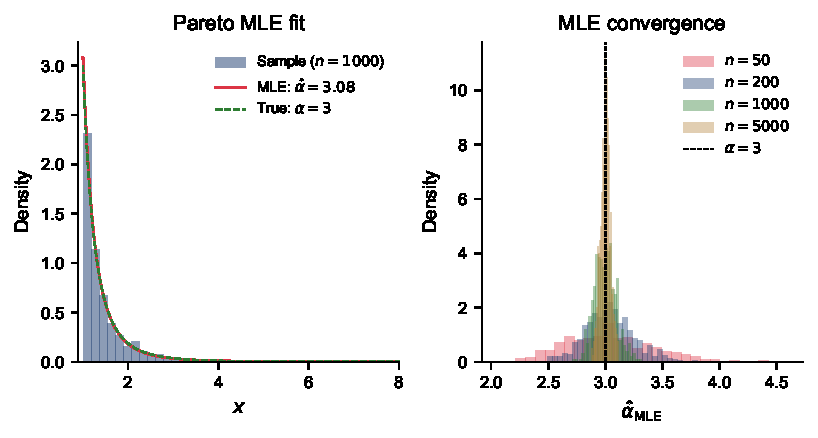
\includegraphics[width=0.72\textwidth]{ch2_pareto_mle_demo.pdf}
\end{center}
\vspace{-0.3cm}
\quantlet{SFM\_ch2\_pareto\_analysis}{https://github.com/QuantLet/Stat_fin_markets/tree/master/SFM_ch2/SFM_ch2_pareto_analysis}
\end{frame}

%--- MSc Slide P2c: Hill estimator pe S&P 500 ---
\slidelevel{MSc}
\begin{frame}{Distribuția Pareto --- Estimatorul Hill pe date reale}
\small
\vspace{-0.2cm}
\begin{center}
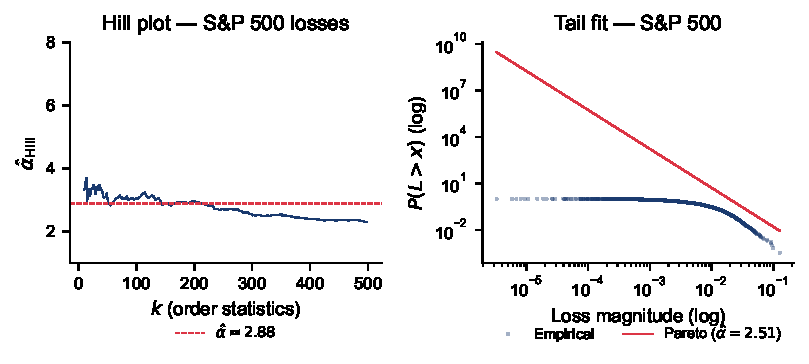
\includegraphics[width=0.82\textwidth]{ch2_pareto_hill_sp500.pdf}
\end{center}
\vspace{-0.3cm}
\quantlet{SFM\_ch2\_pareto\_analysis}{https://github.com/QuantLet/Stat_fin_markets/tree/master/SFM_ch2/SFM_ch2_pareto_analysis}
\begin{columns}[T]
\begin{column}{0.48\textwidth}
\begin{itemize}\setlength\itemsep{1pt}
\item \textbf{Hill plot}: $\hat{\alpha}_{\text{Hill}}$ vs.\ $k$ (nr.\ statistici de ordine)
\item Zona stabilă: $\hat{\alpha} \approx 2{,}9$ pentru pierderile S\&P~500 (2000--2025)
\item $\alpha < 3$ $\Rightarrow$ momente de ordin $\geq 3$ nu există
\end{itemize}
\end{column}
\begin{column}{0.48\textwidth}
\begin{itemize}\setlength\itemsep{1pt}
\item Coada empirică se aliniază bine cu Pareto fitted
\item Pragul optim: echilibru \textit{bias--variance}
\item Confirmare: \textbf{cozi groase} în piețele financiare reale
\end{itemize}
\end{column}
\end{columns}
\end{frame}

%--- MSc Slide P2c2: Tail fitting detaliat ---
\slidelevel{MSc}
\begin{frame}{Distribuția Pareto --- Fitting pe coada distribuției}
\small
\vspace{-0.2cm}
\begin{center}
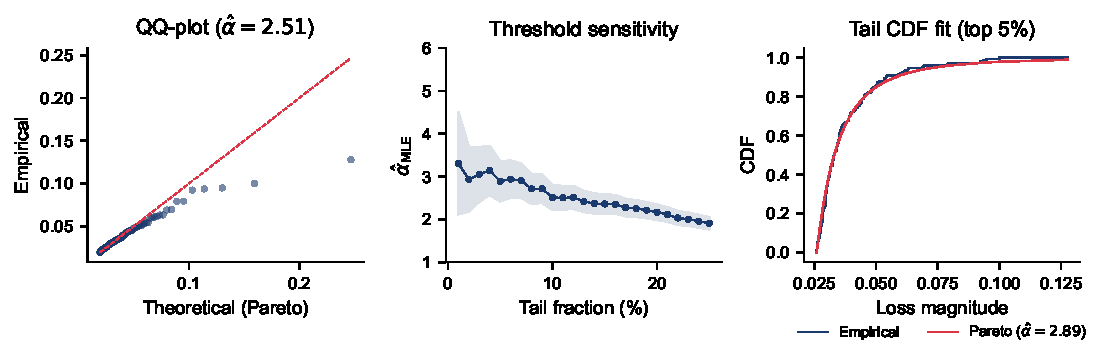
\includegraphics[width=0.92\textwidth]{ch2_pareto_tail_fitting.pdf}
\end{center}
\vspace{-0.3cm}
\quantlet{SFM\_ch2\_pareto\_analysis}{https://github.com/QuantLet/Stat_fin_markets/tree/master/SFM_ch2/SFM_ch2_pareto_analysis}
\begin{itemize}\setlength\itemsep{1pt}
\item \textbf{QQ-plot}: dacă punctele se aliniază pe diagonală $\Rightarrow$ coada este Pareto
\item \textbf{Sensibilitatea pragului}: $\hat{\alpha}$ variază cu fracția de coadă selectată; zona stabilă $\approx$ 3--8\%
\item \textbf{CDF fit}: comparăm CDF-ul empiric al cozii cu CDF-ul Pareto estimat
\item S\&P~500 (2000--2025): $\hat{\alpha} \approx 2{,}5$--$3{,}0$ $\Rightarrow$ momente finite doar până la ordinul 2
\end{itemize}
\end{frame}

%--- Y3 Slide P2d: Aplicații ale distribuției Pareto ---
\slidelevel{Y3}
\begin{frame}{Distribuția Pareto --- Aplicații}
\small
\begin{columns}[T]
\begin{column}{0.48\textwidth}
\begin{block}{Legea lui Zipf (capitalizare de piață)}
\begin{center}
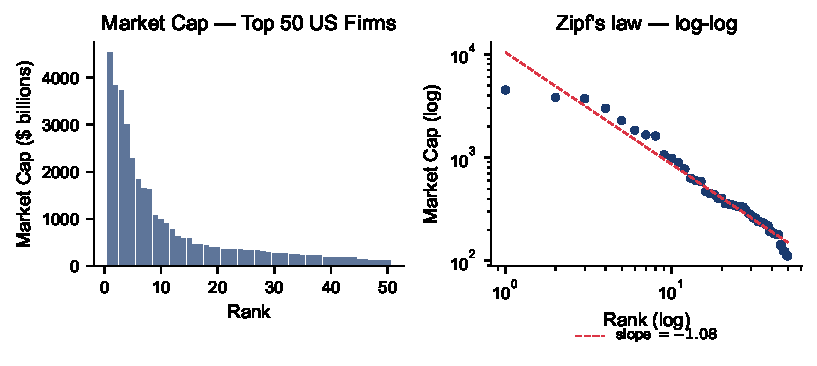
\includegraphics[width=\textwidth]{ch2_pareto_market_cap.pdf}
\end{center}
\vspace{-0.2cm}
\begin{itemize}\setlength\itemsep{1pt}
\item Capitalizarea firmelor urmează o lege de putere
\item Top 10 firme $\approx$ 30\% din piață
\item Panta Zipf $\approx -1$ (lege empirică universală)
\end{itemize}
\end{block}
\end{column}
\begin{column}{0.48\textwidth}
\begin{block}{Alte aplicații ale distribuției Pareto}
\begin{itemize}\setlength\itemsep{2pt}
\item \textbf{Pierderi din asigurări}: sumele asigurate extreme $\Rightarrow$ Pareto
\item \textbf{Riscul operațional} (Basel~II): pierderile operaționale au coada Pareto
\item \textbf{Distribuția averii}: Top 1\% deține 40--50\% din avere (Piketty, 2014)
\item \textbf{Volumul tranzacțiilor}: câteva tranzacții mari domină volumul total
\item \textbf{Cyber risk}: severitatea atacurilor cibernetice este Pareto-distribuită
\end{itemize}
\end{block}
\end{column}
\end{columns}
\end{frame}

%--- MSc Slide P3 ---
\slidelevel{MSc}
\begin{frame}{Distribuția Pareto --- Conexiuni teoretice}
\small
\vspace{-0.3cm}
\begin{block}{Legătura cu EVT și estimatorul Hill}
\begin{itemize}\setlength\itemsep{1pt}
\item \textbf{Teorema Pickands--Balkema--de Haan}: excedentele peste un prag suficient de mare urmează aproximativ o \textbf{distribuție Pareto generalizată} (GPD)
\item Distribuția Pareto clasică = caz particular al GPD cu $\xi > 0$
\item \textbf{Estimatorul Hill}: estimează $\alpha$ din statisticile de ordine $X_{(1)} \leq \cdots \leq X_{(n)}$:
\[
\hat{\alpha}_{\text{Hill}} = \left(\frac{1}{k}\sum_{i=1}^{k} \ln \frac{X_{(n-i+1)}}{X_{(n-k)}}\right)^{-1}
\]
\end{itemize}
\end{block}

\begin{block}{Legătura cu distribuțiile stabile și Student-$t$}
\begin{itemize}\setlength\itemsep{1pt}
\item Distribuțiile $\alpha$-stabile cu $\alpha < 2$ au cozi Pareto: $P(X > x) \sim C_\alpha\, x^{-\alpha}$
\item Student-$t$ cu $\nu$ grade de libertate: cozi Pareto cu indice $\alpha = \nu$
\item Indicele de coadă Pareto unifică teoria: mai mic $\alpha$ $\Rightarrow$ cozi mai groase
\end{itemize}
\end{block}
\end{frame}

%=============================================================================
% ACTUALIZARE CUPRINS după Secțiunea 5
%=============================================================================
{
\setbeamertemplate{headline}{%
    \vskip10pt%
    \hbox to \paperwidth{\hskip0.5cm\hfill\hskip0.5cm}%
    \vskip4pt%
    {\color{FooterGray}\hrule height 0.4pt}%
}
\begin{frame}{}
    {\color{FooterGray}\hrule height 0.4pt}
    \vspace{0.1cm}
    {\Large\textcolor{IDAred}{\textbf{Cuprins}}}
    \vspace{0.2cm}
    {\small
    \begin{columns}[T]
        \begin{column}{0.48\textwidth}
            \begin{itemize}
                \item Introducere \checkmark
                \item De la prețuri la log-randamente \checkmark
                \item Distribuția normală \checkmark
                \item Fapte stilizate \checkmark
                \item Distribuția Student-$t$ \checkmark
                \item Distribuția Pareto \checkmark
                \item \textbf{Distribuții asimetrice}
            \end{itemize}
        \end{column}
        \begin{column}{0.48\textwidth}
            \begin{itemize}
                \item Distribuții stabile
                \item Teoria valorilor extreme
                \item Comparația distribuțiilor
                \item Copule și dependența de coadă (\textit{tail dependence})
                \item Managementul riscului
                \item Extensii moderne / Rezumat
            \end{itemize}
        \end{column}
    \end{columns}
    }
\end{frame}
}

%=============================================================================
% SECȚIUNEA 6: DISTRIBUȚII ASIMETRICE
%=============================================================================

%=============================================================================
% SECȚIUNEA 7: STUDIU DE CAZ
%=============================================================================
\section{Studiu de caz}

%--- Y3 Slide 1: Datele ---
\slidelevel{Y3}
\begin{frame}{Studiu de caz: Datele}
\quantlet{SFM\_ch2\_case\_study\_2a}{https://github.com/QuantLet/Stat_fin_markets/tree/master/Ch_02/SFM_ch2_case_study_2a}
    \begin{columns}[T]
        \begin{column}{0.55\textwidth}
            \begin{block}{Prețuri și log-randamente}
            \small
            Analizăm trei active cu caractere diferite:
            \begin{itemize}
                \item \textcolor{MainBlue}{\textbf{S\&P 500}} — piață dezvoltată, lichiditate mare
                \item \textcolor{IDAred}{\textbf{BRD}} — acțiune românească, piață emergentă
                \item \textcolor{Forest}{\textbf{Bitcoin}} — activ digital, volatilitate extremă
            \end{itemize}
            Perioadă: 2015--2025, date zilnice.
            \end{block}
        \end{column}
        \begin{column}{0.42\textwidth}
            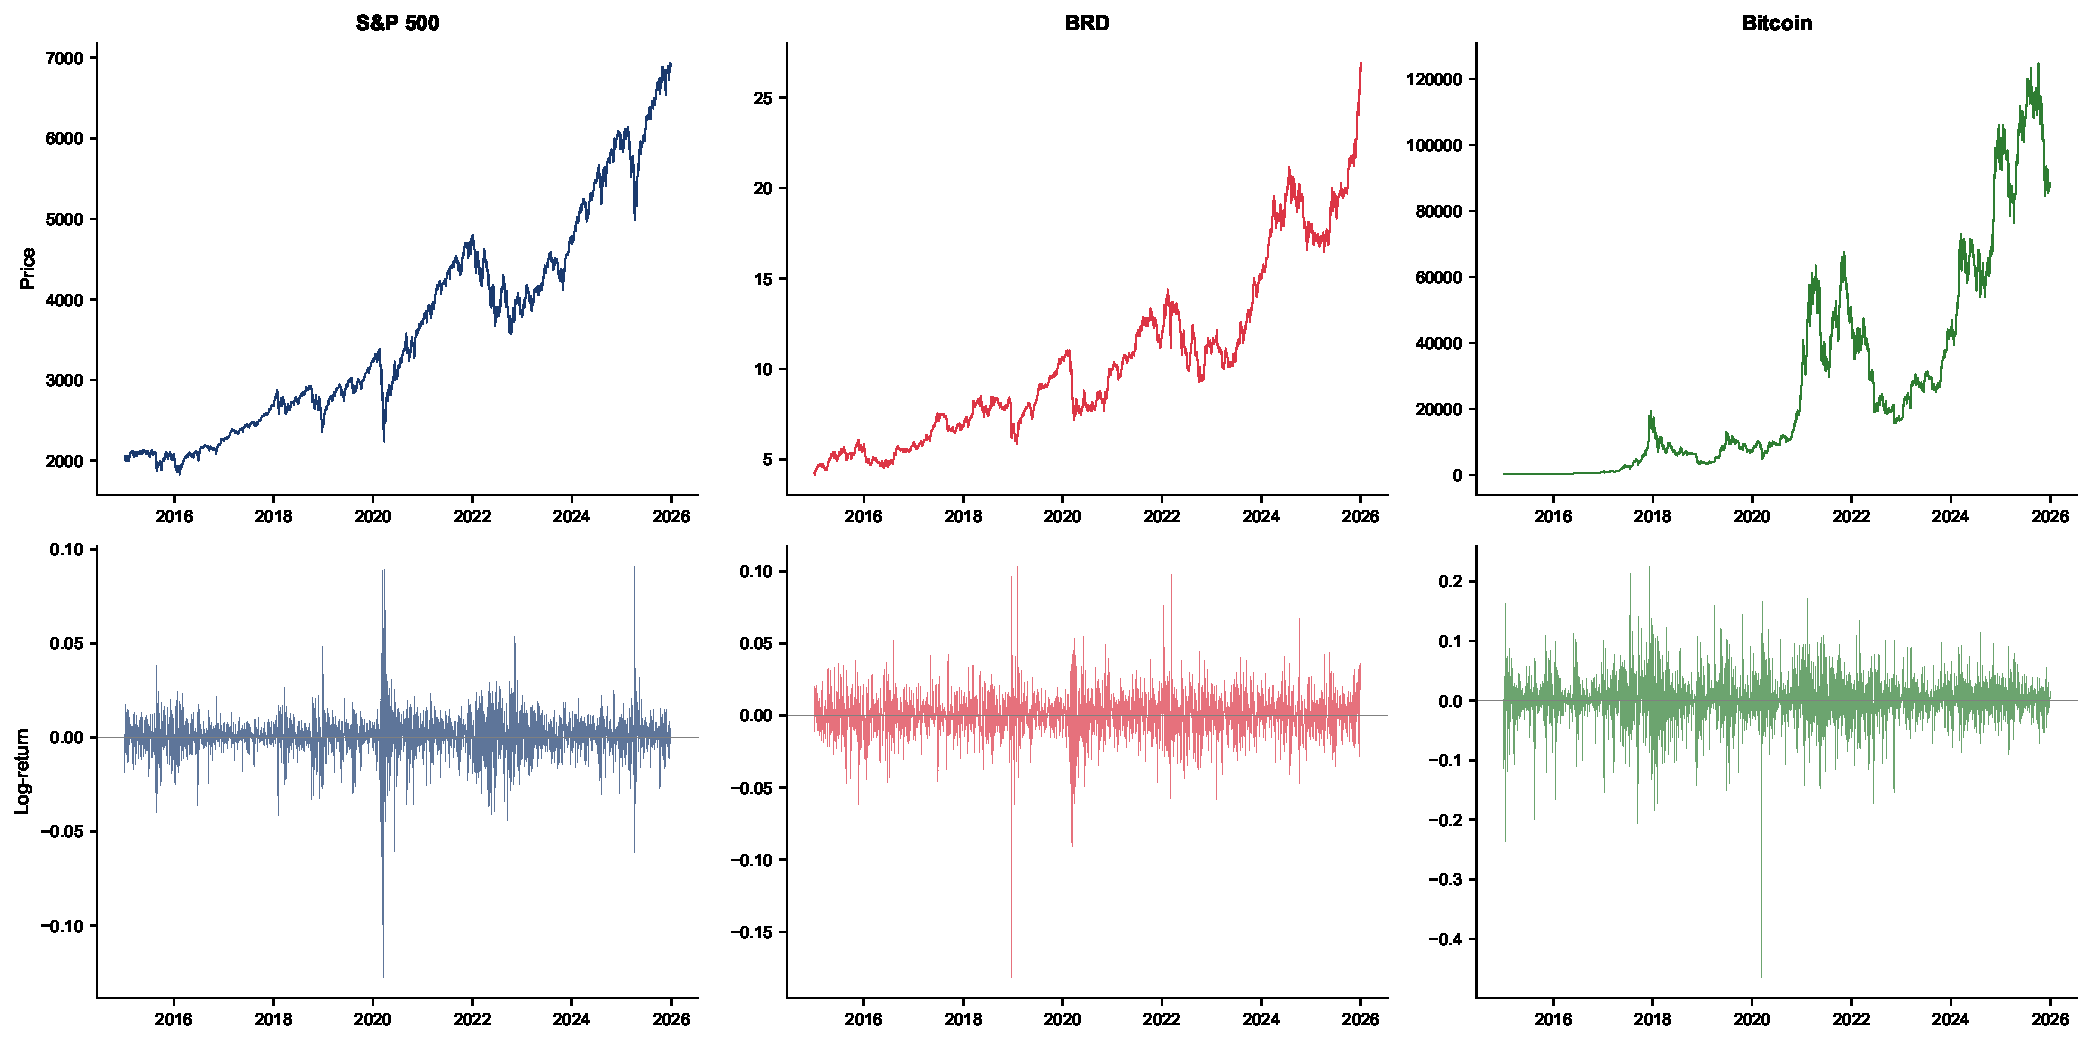
\includegraphics[width=\textwidth]{../../charts/ch2_cs2a_price_returns.pdf}
        \end{column}
    \end{columns}

    \vspace{0.2cm}
    {\scriptsize
    \begin{tabular}{lrrrrr}
    \toprule
    \textbf{Activ} & \textbf{N} & \textbf{Media (\%)} & \textbf{Std (\%)} & \textbf{Skew} & \textbf{Kurt} \\
    \midrule
    S\&P 500 & $\sim$2\,500 & 0.05 & 1.15 & $-$0.60 & 13.5 \\
    BRD      & $\sim$2\,500 & 0.04 & 1.10 & $-$0.80 & 12.0 \\
    Bitcoin   & $\sim$3\,600 & 0.12 & 3.80 & $-$0.30 & 8.5 \\
    \bottomrule
    \end{tabular}}
\end{frame}

%--- Y3 Slide 2: Fapte stilizate ---
\slidelevel{Y3}
\begin{frame}{Studiu de caz: Fapte stilizate}
    \begin{columns}[T]
        \begin{column}{0.55\textwidth}
            \begin{block}{Volatilitate clusterizată}
            \small
            ACF a $|r_t|$ confirmă dependența pe termen lung:
            \begin{itemize}
                \item Toate cele 3 active prezintă autocorelație semnificativă a $|r_t|$ până la lag-ul 60
                \item \textbf{Kurtosis} $\gg 3$ pe toate piețele $\Rightarrow$ cozi groase
                \item \textbf{Asimetrie negativă} pentru S\&P 500 și BRD (\emph{leverage effect})
                \item Bitcoin: asimetrie mai redusă, dar volatilitate de 3$\times$
            \end{itemize}
            \end{block}
        \end{column}
        \begin{column}{0.42\textwidth}
            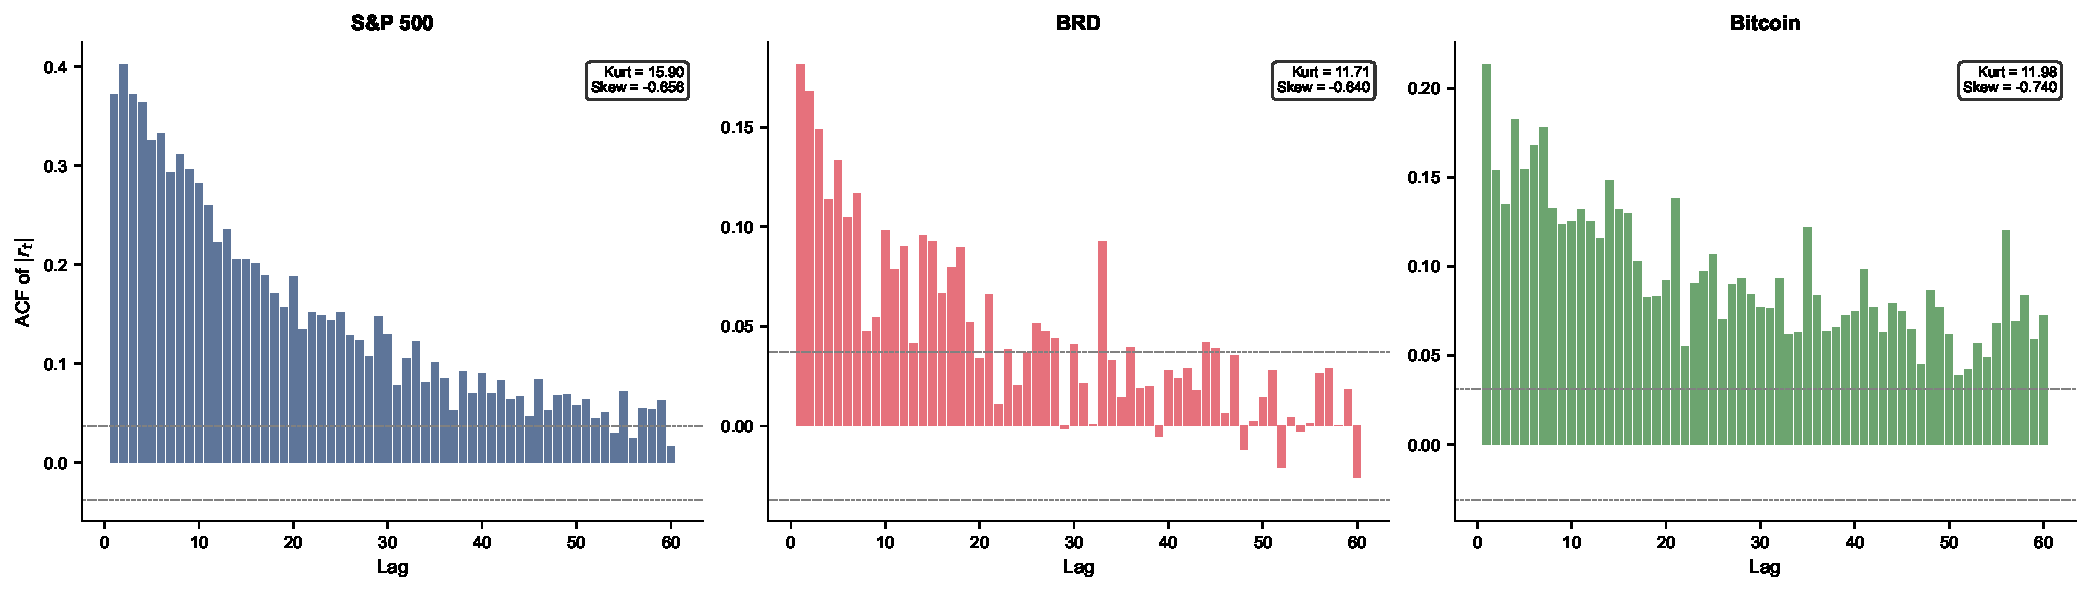
\includegraphics[width=\textwidth]{../../charts/ch2_cs2a_stylized_3assets.pdf}
        \end{column}
    \end{columns}

    \begin{rmk}
    \begin{itemize}
    \item Clusterizarea volatilității invalidează ipoteza i.i.d. necesară modelului Black--Scholes
    \end{itemize}
    \end{rmk}
\end{frame}

%--- Y3 Slide 3: Normal vs Student-t ---
\slidelevel{Y3}
\begin{frame}{Studiu de caz: Normal vs Student-t}
\quantlet{SFM\_ch2\_case\_study\_2a}{https://github.com/QuantLet/Stat_fin_markets/tree/master/Ch_02/SFM_ch2_case_study_2a}
    \begin{columns}[T]
        \begin{column}{0.55\textwidth}
            \begin{block}{Histogramă log-scale cu overlay}
            \small
            Comparam cele două modele pe scara logaritmică:
            \begin{itemize}
                \item \textcolor{MainBlue}{Normal} subestimează sistematic cozile
                \item \textcolor{IDAred}{Student-t} se adaptează bine cu $\nu$ estimat:
                \begin{itemize}
                    \item S\&P 500: $\hat{\nu} \approx 4$--$5$
                    \item BRD: $\hat{\nu} \approx 3$--$5$
                    \item Bitcoin: $\hat{\nu} \approx 3$--$4$
                \end{itemize}
                \item Diferența crește exponențial în cozi
            \end{itemize}
            \end{block}
        \end{column}
        \begin{column}{0.42\textwidth}
            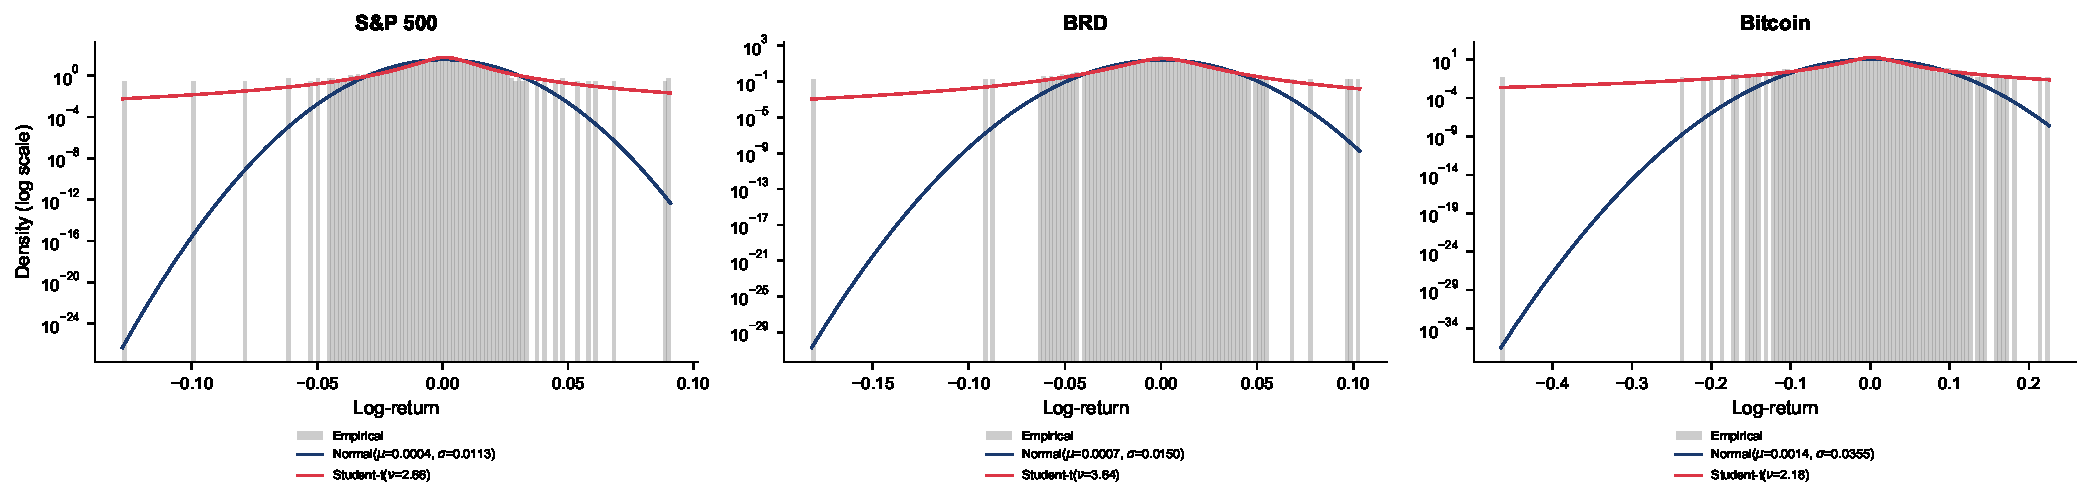
\includegraphics[width=\textwidth]{../../charts/ch2_cs2a_fit_comparison.pdf}
        \end{column}
    \end{columns}
\end{frame}

%--- Y3 Slide 4: QQ-plots ---
\slidelevel{Y3}
\begin{frame}{Studiu de caz: QQ-plots}
    \begin{center}
        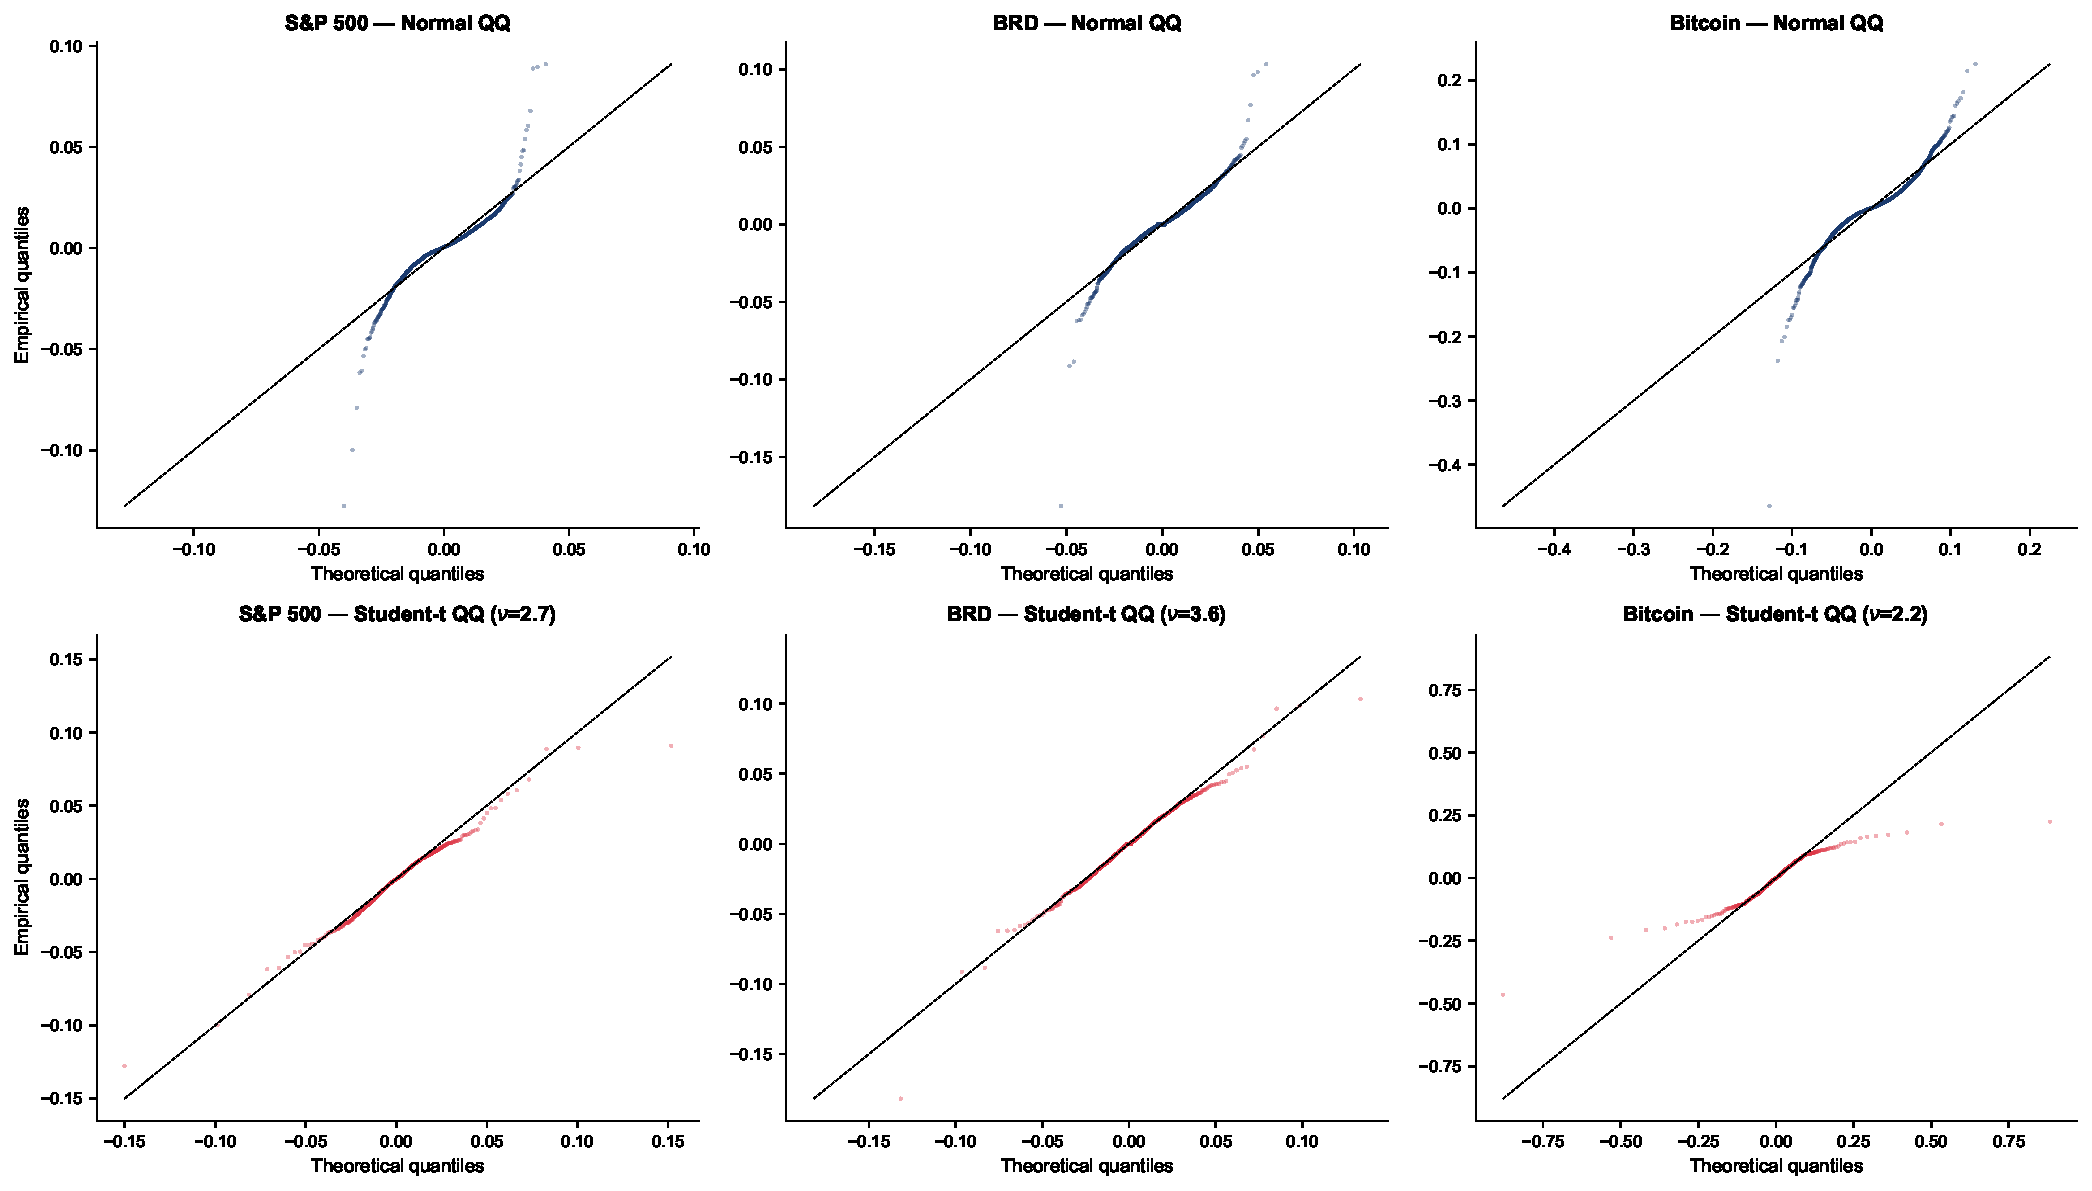
\includegraphics[width=0.65\textwidth]{../../charts/ch2_cs2a_qq_comparison.pdf}
    \end{center}
    \vspace{-0.4cm}
    {\footnotesize
    \begin{itemize}\setlength{\itemsep}{0pt}
        \item \textbf{Normal QQ}: deviații sistematice în cozi \quad \textbf{Student-t QQ}: aliniere mult mai bună
        \item Bitcoin: cele mai mari deviații, confirmând cozi mai groase
    \end{itemize}}
\end{frame}

%--- Y3 Slide 5: Teste de normalitate ---
\slidelevel{Y3}
\begin{frame}{Studiu de caz: Teste de normalitate}
    \begin{block}{Testarea ipotezei $H_0$: randamentele $\sim \mathcal{N}(\mu, \sigma^2)$}
    \small
    {\centering
    \begin{tabular}{lrrrr}
    \toprule
    \textbf{Activ} & \textbf{Jarque--Bera} & \textbf{Shapiro--Wilk} & \textbf{Anderson--Darling} & \textbf{Kolmogorov--Smirnov} \\
    \midrule
    S\&P 500 & $> 10\,000^{***}$ & $< 0.99^{***}$ & $> 20^{***}$ & $> 0.05^{***}$ \\
    BRD      & $> 8\,000^{***}$  & $< 0.99^{***}$ & $> 15^{***}$ & $> 0.04^{***}$ \\
    Bitcoin  & $> 5\,000^{***}$  & $< 0.98^{***}$ & $> 30^{***}$ & $> 0.06^{***}$ \\
    \bottomrule
    \end{tabular}\par}
    \vspace{0.2cm}
    $^{***}$ respingere la nivel $\alpha = 0.001$ pentru toate testele și toate activele.
    \end{block}

    \begin{alertblock}{Concluzie}
        \begin{itemize}
            \item Normalitatea este \textbf{respinsă decisiv} pe toate cele trei piețe
            \item Cele patru teste converg: JB (momente), SW (ordine), AD (cozi), KS (distribuție completă)
        \end{itemize}
    \end{alertblock}
\end{frame}

%--- Y3 Slide 5b: VaR/ES --- Cuantificarea riscului ---
\slidelevel{Y3}
\begin{frame}{Studiu de caz: VaR și ES --- Normal vs Student-$t$}
    \begin{block}{Aplicarea formulelor de risc (portofoliu 1M EUR, $\mu \approx 0$)}
    \small
    Formule: $\text{VaR}^{N}_{1\%} = 2{,}326\,\sigma$; \quad $\text{VaR}^{t}_{1\%} = \sqrt{\tfrac{\nu-2}{\nu}}\,|t_\nu^{-1}(0{,}01)|\,\sigma$; \quad ES: media cozii stângi sub $\text{VaR}$.
    \vspace{0.1cm}

    {\centering
    \renewcommand{\arraystretch}{1.05}
    \footnotesize
    \begin{tabular}{lrrrr}
    \toprule
    \textbf{Activ} ($\sigma$, $\hat{\nu}$) & \textbf{VaR Normal} & \textbf{VaR Student-$t$} & \textbf{ES Normal} & \textbf{ES Student-$t$} \\
    \midrule
    S\&P 500 ($1{,}15\%$, $4{,}5$) & 26\,750 & 30\,400 & 30\,500 & 40\,200 \\
    BRD ($1{,}10\%$, $3{,}8$)       & 25\,590 & 29\,600 & 29\,300 & 40\,200 \\
    Bitcoin ($3{,}80\%$, $3{,}2$)    & 88\,390 & 102\,000 & 100\,900 & 148\,700 \\
    \bottomrule
    \end{tabular}\par}
    \end{block}

    \begin{alertblock}{ES Normal subestimează cu 30--50\%}
    \begin{itemize}
        \item $P(r < -3\sigma)$: Normal $= \Phi(-3) = 0{,}135\%$ (1 zi/741); \quad Student-$t$ ($\hat{\nu}\!=\!4{,}5$) $\approx 0{,}58\%$ (1 zi/172) --- de $\mathbf{4{,}3\times}$ mai frecvent
    \end{itemize}
    \end{alertblock}
\end{frame}

%--- Y3 Slide 5c: AIC/BIC ---
\slidelevel{Y3}
\begin{frame}{Studiu de caz: Selecția modelului --- AIC/BIC}
    \begin{block}{Criterii informaționale ($\text{AIC} = -2\ell + 2k$; \; $\text{BIC} = -2\ell + k\ln n$)}
    \small
    {\centering
    \renewcommand{\arraystretch}{1.1}
    \begin{tabular}{lccc}
    \toprule
    \textbf{Activ} & \textbf{$\Delta$AIC (Normal $-$ Student-$t$)} & \textbf{$\Delta$BIC} & \textbf{Câștigător} \\
    \midrule
    S\&P 500 & $> 200$ & $> 190$ & Student-$t$ \\
    BRD      & $> 150$ & $> 140$ & Student-$t$ \\
    Bitcoin  & $> 300$ & $> 290$ & Student-$t$ \\
    \bottomrule
    \end{tabular}\par}
    \end{block}

    \begin{rmk}
    \begin{itemize}
    \item $\Delta\text{AIC} > 10$ $\Rightarrow$ evidență puternică împotriva modelului Normal (Burnham \& Anderson)
    \item Student-$t$ câștigă decisiv pe toate piețele, deși are un parametru suplimentar ($\nu$)
    \end{itemize}
    \end{rmk}
\end{frame}

%--- Y3 Slide 6: Concluzii ---
\slidelevel{Y3}
\begin{frame}{Studiu de caz: Concluzii}
    \begin{block}{Lecții din analiza datelor reale}
    \small
    \begin{enumerate}
        \item \textbf{Kurtosis} $\gg 3$ pe toate piețele $\Rightarrow$ modelul Normal este inadecvat
        \item \textbf{Student-t} oferă o primă aproximare, dar are \emph{cozi simetrice}
        \item \textbf{Asimetria} (mai ales pe S\&P 500 și BRD) necesită modele asimetrice
        \item \textbf{Volatilitatea clusterizată} cere modele condiționale (GARCH)
    \end{enumerate}
    \end{block}

    \begin{alertblock}{Implicații pentru managementul riscului}
        ES Normal la 1\% subestimează pierderea medie din coadă cu \textbf{30--50\%} față de Student-$t$ (cf.\ tabelul anterior). VaR Normal subestimează cu $\sim$15\%, dar evenimentele de $3\sigma$ apar de $4\times$ mai des.
    \end{alertblock}

    \begin{rmk}
    \begin{itemize}
    \item \textbf{Capitolul 3} introduce distribuții cu \emph{cozi groase}: stabilă, skew-t, GED, EVT
    \end{itemize}
    \end{rmk}
\end{frame}

%=============================================================================
% SECTIUNEA: QUIZ
%=============================================================================
\section{Quiz}
\slidelevel{Y3}
\begin{frame}{Întrebarea 1}
    \begin{cminipage}{0.95\textwidth}
    \begin{alertblock}{Întrebare}
        \begin{itemize}
            \item Evenimentul din 19 octombrie 1987 (S\&P~500 $-20{,}5\%$) corespunde unui eveniment de $\sim$20$\sigma$ sub ipoteza normală ($\sigma \approx 1\%$). Care este probabilitatea unui astfel de eveniment?
        \end{itemize}
    \end{alertblock}

    \vspace{0.3cm}

    \begin{block}{Variante de răspuns}

        \textcolor{MainBlue}{\textbf{(A)}} $\approx 10^{-2}$ (1 la 100)\\[3pt]

        \textcolor{MainBlue}{\textbf{(B)}} $\approx 10^{-30}$ (practic imposibil pe orizontul uman)\\[3pt]

        \textcolor{MainBlue}{\textbf{(C)}} $\approx 10^{-89}$ (imposibil în durata de viață a universului)\\[3pt]

        \textcolor{MainBlue}{\textbf{(D)}} $\approx 10^{-6}$ (o dată la un milion de zile)

    \end{block}
    \end{cminipage}
\end{frame}

\slidelevel{Y3}
\begin{frame}{Întrebarea 1: Răspuns}
    \begin{cminipage}{0.95\textwidth}
    \begin{exampleblock}{Răspuns: (C)}
    \begin{itemize}
        \item Sub distribuția normală ($\sigma \approx 1\%$), un eveniment de $\sim$20$\sigma$ are probabilitatea $\approx 10^{-89}$.
        \item Și totuși s-a întâmplat --- aceasta demonstrează \textbf{inadecvarea distribuției normale} pentru evenimente extreme.
        \item Sub distribuții cu cozi groase (Student-$t$, stabilă), astfel de evenimente au probabilități mult mai mari.
        \item Aceasta este motivația principală pentru studierea distribuțiilor alternative.
    \end{itemize}
    \end{exampleblock}
    \end{cminipage}
\end{frame}

\slidelevel{Y3}
\begin{frame}{Întrebarea 2}
    \begin{cminipage}{0.95\textwidth}
    \begin{alertblock}{Întrebare}
        \begin{itemize}
            \item O distribuție Student-$t$ cu $\nu = 4$ grade de libertate are:
        \end{itemize}
    \end{alertblock}

    \vspace{0.3cm}

    \begin{block}{Variante de răspuns}

        \textcolor{MainBlue}{\textbf{(A)}} Medie finită, varianță finită, kurtosis finită\\[3pt]

        \textcolor{MainBlue}{\textbf{(B)}} Medie finită, varianță finită, kurtosis infinită\\[3pt]

        \textcolor{MainBlue}{\textbf{(C)}} Medie finită, varianță infinită, kurtosis infinită\\[3pt]

        \textcolor{MainBlue}{\textbf{(D)}} Medie infinită, varianță infinită, kurtosis infinită

    \end{block}
    \end{cminipage}
\end{frame}

\slidelevel{Y3}
\begin{frame}{Întrebarea 2: Răspuns}
    \begin{cminipage}{0.95\textwidth}
    \begin{exampleblock}{Răspuns: (B)}
    \begin{itemize}
        \item Pentru Student-$t$: media există dacă $\nu > 1$, varianța dacă $\nu > 2$, kurtosis dacă $\nu > 4$.
        \item Cu $\nu = 4$: media finită (\checkmark), varianță finită ($= \nu/(\nu-2) = 2$, \checkmark), dar kurtosis-ul \textbf{nu există} (momentul de ordin 4 diverge: $6/(\nu-4)$ cu $\nu=4$).
        \item (A) este greșit: momentul de ordin 4 nu există la $\nu = 4$ exact.
        \item Aceasta arată că și distribuțiile cu varianță finită pot avea cozi \textbf{foarte groase}.
    \end{itemize}
    \end{exampleblock}
    \end{cminipage}
\end{frame}

%=============================================================================
% SECTIUNEA: EXERCITII DE EXAMEN
%=============================================================================
\section{Exercitii de examen}
\slidelevel{Y3}
\begin{frame}{Exercițiul 1: Log-randamente și momente}
\begin{block}{Enunț}
Se dau prețurile zilnice de închidere:
\begin{center}
{\small
\renewcommand{\arraystretch}{1.2}
\begin{tabular}{lccccc}
\toprule
$t$ & 0 & 1 & 2 & 3 & 4 \\
\midrule
$P_t$ & 100 & 103 & 98 & 95 & 102 \\
\bottomrule
\end{tabular}
}
\end{center}
\end{block}
\begin{enumerate}
    \item Calculați log-randamentele $r_t = \ln(P_t/P_{t-1})$ pentru $t = 1, \ldots, 4$.
    \item Calculați media, varianța, asimetria și kurtosis eșantionului.
    \item Aplicați testul Jarque--Bera: $JB = \frac{n}{6}\left(S^2 + \frac{(K-3)^2}{4}\right)$. Se respinge normalitatea la 5\%?
    \item Calculați log-randamentul total pe 4 perioade. Verificați aditivitatea temporală.
\end{enumerate}
\end{frame}

\slidelevel{Y3}
\begin{frame}{Exercițiul 2: Distribuția normală și VaR}
\begin{block}{Enunț}
Un portofoliu de \$5M are randamente zilnice $\sim N(\mu, \sigma^2)$ cu $\hat{\mu} = 0{,}04\%$ și $\hat{\sigma} = 1{,}2\%$.
\end{block}
\begin{enumerate}
    \item Calculați VaR zilnic la nivelurile 5\%, 1\% și 0{,}1\%.
    \item Calculați Expected Shortfall la nivelul 1\%.
    \item Un eveniment de $-4\%$ a avut loc. Ce probabilitate are sub ipoteza normală?
    \item Argumentați de ce VaR normal poate subestima riscul real.
\end{enumerate}
\vspace{0.1cm}
\begin{exampleblock}{Indiciu}
$\text{VaR}_\alpha = -(\mu + z_\alpha \cdot \sigma)$, unde $z_{0{,}05} = -1{,}645$, $z_{0{,}01} = -2{,}326$, $z_{0{,}001} = -3{,}090$.
\end{exampleblock}
\end{frame}

\slidelevel{Y3}
\begin{frame}{Exercițiul 3: Student-$t$ --- Ajustare și comparație}
\begin{block}{Enunț}
Pe datele de la Exercițiul 1, presupuneți că MLE produce: distribuția normală $\ell = 12{,}5$, Student-$t$ ($\nu = 5$) $\ell = 14{,}8$.
\end{block}
\begin{enumerate}
    \item Calculați AIC și BIC pentru ambele modele ($k_N = 2$, $k_t = 3$, $n = 4$).
    \item Care model este preferat de AIC? Dar de BIC?
    \item Calculați excesul de kurtosis (\textit{excess kurtosis}) al distribuției Student-$t$ cu $\nu = 5$.
    \item Explicați de ce Student-$t$ captează mai bine cozile groase decât distribuția normală.
\end{enumerate}
\vspace{0.1cm}
\begin{alertblock}{Formule}
$\text{AIC} = -2\ell + 2k$, \quad $\text{BIC} = -2\ell + k\ln n$, \quad $\kappa = 6/(\nu - 4)$ pentru $\nu > 4$.
\end{alertblock}
\end{frame}

%=============================================================================
% LABORATOR PYTHON
%=============================================================================

\slidelevel{Y3}
\begin{frame}{Laborator Python --- Exerciții interactive}
\small
\begin{block}{Lab 1: Ajustarea distribuțiilor (Y3)}
Deschideți \texttt{SFM\_ch2\_normal\_distribution.ipynb}:
\begin{enumerate}
\item Descărcați date S\&P~500 (2015--2025); calculați log-randamentele
\item Histogramă + suprapunere normală; testul Jarque--Bera
\item Ajustați Student-$t$ (MLE). Comparați AIC cu modelul normal
\end{enumerate}
\end{block}
\quantlet{SFM\_ch2\_normal\_distribution}{https://github.com/QuantLet/Stat_fin_markets/tree/master/Ch_02/SFM_ch2_normal_distribution}
\end{frame}

%=============================================================================
% REZOLVARI EXERCITII
%=============================================================================
\section*{Rezolvări exerciții}
\slidelevel{Y3}
\begin{frame}{Exercițiul 1: Rezolvare}
\begin{block}{Rezolvare}
\textbf{1.} Log-randamente: $r_1 = \ln(103/100) = 0{,}0296$, $r_2 = \ln(98/103) = -0{,}0498$, $r_3 = \ln(95/98) = -0{,}0311$, $r_4 = \ln(102/95) = 0{,}0713$.

\textbf{2.} $\bar{r} = (0{,}0296 - 0{,}0498 - 0{,}0311 + 0{,}0713)/4 = 0{,}0050$; \;$s^2 = \frac{1}{3}\sum(r_i - \bar{r})^2 = 0{,}00253$; \;$s = 0{,}0503$.

Asimetrie: $S = \frac{n}{(n-1)(n-2)}\sum\!\left(\frac{r_i - \bar{r}}{s}\right)^3 \approx 0{,}56$; \;Kurtosis: $K \approx 1{,}72$.

\textbf{3.} $JB = \frac{4}{6}(0{,}56^2 + (1{,}72-3)^2/4) = 0{,}21 + 0{,}27 = 0{,}48$. Cu $\chi^2_2(0{,}05) = 5{,}99$: $0{,}48 < 5{,}99$ $\Rightarrow$ \textbf{nu respingem} normalitatea (eșantion prea mic!).

\textbf{4.} $r_{0:4} = \ln(102/100) = 0{,}0198 = r_1 + r_2 + r_3 + r_4 = 0{,}0198$ \checkmark
\end{block}
\end{frame}

\slidelevel{Y3}
\begin{frame}{Exercițiul 2: Rezolvare}
\begin{block}{Rezolvare}
Date: $\mu = 0{,}0004$, $\sigma = 0{,}012$, portofoliu \$5M.

\textbf{1.} $\text{VaR}_\alpha = -(\mu + z_\alpha\sigma) \times W$
\begin{itemize}
\item VaR 5\%: $-(0{,}0004 + (-1{,}645)(0{,}012)) \times 5\text{M} = 0{,}01934 \times 5\text{M} = \$96.680$
\item VaR 1\%: $-(0{,}0004 + (-2{,}326)(0{,}012)) \times 5\text{M} = 0{,}02751 \times 5\text{M} = \$137.560$
\item VaR 0{,}1\%: $-(0{,}0004 + (-3{,}090)(0{,}012)) \times 5\text{M} = 0{,}03668 \times 5\text{M} = \$183.400$
\end{itemize}

\textbf{2.} $\text{ES}_{1\%} = \sigma \cdot \phi(-2{,}326)/0{,}01 = 0{,}012 \times 0{,}02665/0{,}01 = 0{,}03198$ $\Rightarrow$ \$159.900

\textbf{3.} $P(r < -0{,}04) = \Phi\!\left(\frac{-0{,}04 - 0{,}0004}{0{,}012}\right) = \Phi(-3{,}37) \approx 0{,}038\%$ (1 zi în $\sim$2.600)

\textbf{4.} Empiric, evenimentele $> 3\sigma$ apar mult mai frecvent $\Rightarrow$ VaR sub distribuția normală subestimează riscul.
\end{block}
\end{frame}

\slidelevel{Y3}
\begin{frame}{Exercițiul 3: Rezolvare}
\begin{block}{Rezolvare}
Date: $\ell_N = 12{,}5$, $\ell_t = 14{,}8$, $k_N = 2$, $k_t = 3$, $n = 4$.

\textbf{1.}
\begin{itemize}
\item Distribuția normală: AIC $= -2(12{,}5) + 2(2) = -21{,}0$; \;BIC $= -25 + 2\ln 4 = -25 + 2{,}77 = -22{,}23$
\item Student-$t$: AIC $= -2(14{,}8) + 2(3) = -23{,}6$; \;BIC $= -29{,}6 + 3\ln 4 = -29{,}6 + 4{,}16 = -25{,}44$
\end{itemize}

\textbf{2.} Student-$t$ câștigă pe ambele criterii (AIC: $-23{,}6 < -21{,}0$; BIC: $-25{,}44 < -22{,}23$).

\textbf{3.} Exces de kurtosis: $\kappa = 6/(\nu - 4) = 6/(5-4) = 6$. Kurtosis totală: $3 + 6 = 9$.

\textbf{4.} PDF-ul Student-$t$ scade ca $|x|^{-(\nu+1)}$ (lege putere) vs.\ $e^{-x^2/2}$ pentru distribuția normală. Decăderea mai lentă alocă mai multă probabilitate în cozi.
\end{block}
\end{frame}

%=============================================================================
% SECȚIUNEA: BIBLIOGRAFIE
%=============================================================================
\section{Bibliografie}

\begin{frame}{Bibliografie I}
    \begin{cminipage}{0.95\textwidth}
    \begin{block}{Manuale de referință}
        {\small
        \begin{itemize}\setlength{\itemsep}{0pt}
            \item McNeil, A., Frey, R. \& Embrechts, P. (2015). \textit{Quantitative Risk Management}. Princeton University Press.
            \item Nolan, J. P. (2020). \textit{Stable Distributions --- Models for Heavy Tailed Data}. Birkh\"{a}user.
            \item Rachev, S. T. (2003). \textit{Handbook of Heavy Tailed Distributions in Finance}. Elsevier.
        \end{itemize}
        }
    \end{block}

    \begin{exampleblock}{Articole fundamentale}
        {\small
        \begin{itemize}\setlength{\itemsep}{0pt}
            \item Mandelbrot, B. (1963). The Variation of Certain Speculative Prices. \textit{Journal of Business}, 36(4), 394--419.
            \item Fama, E. (1965). The Behavior of Stock-Market Prices. \textit{Journal of Business}, 38(1), 34--105.
            \item Cont, R. (2001). Empirical Properties of Asset Returns. \textit{Quantitative Finance}, 1(2), 223--236.
        \end{itemize}
        }
    \end{exampleblock}
    \end{cminipage}
\end{frame}

\begin{frame}{Bibliografie II}
    \vspace{-0.3cm}
    \begin{cminipage}{0.95\textwidth}
    \begin{block}{Distribuții și estimare}
        {\small
        \begin{itemize}\setlength{\itemsep}{0pt}
            \item Hansen, B. (1994). Autoregressive Conditional Density Estimation. \textit{International Economic Review}, 35(3), 705--730.
            \item Nolan, J. P. (1997). Numerical Calculation of Stable Densities and Distribution Functions. \textit{Stochastic Models}, 13(4), 759--774.
            \item Barndorff-Nielsen, O. (1977). Exponentially Decreasing Distributions for the Logarithm of Particle Size. \textit{Proc.\ Royal Society A}, 353, 401--419.
        \end{itemize}
        }
    \end{block}

    \begin{exampleblock}{Modele dinamice}
        {\small
        \begin{itemize}\setlength{\itemsep}{0pt}
            \item Hamilton, J. D. (1989). A New Approach to the Economic Analysis of Nonstationary Time Series. \textit{Econometrica}, 57(2), 357--384.
            \item Merton, R. (1976). Option Pricing When Underlying Stock Returns Are Discontinuous. \textit{J.\ of Financial Economics}, 3, 125--144.
            \item Barndorff-Nielsen, O. \& Shephard, N. (2001). Non-Gaussian Ornstein--Uhlenbeck-Based Models. \textit{JRSS B}, 63(2), 167--241.
        \end{itemize}
        }
    \end{exampleblock}
    \end{cminipage}
\end{frame}

\begin{frame}{Bibliografie III}
    \begin{cminipage}{0.95\textwidth}
    \begin{block}{Testare și selecție de modele}
        {\small
        \begin{itemize}\setlength{\itemsep}{0pt}
            \item Vuong, Q. H. (1989). Likelihood Ratio Tests for Model Selection and Non-Nested Hypotheses. \textit{Econometrica}, 57(2), 307--333.
            \item Fissler, T. \& Ziegel, J. F. (2016). Higher Order Elicitability and Osband's Principle. \textit{Annals of Statistics}, 44(4), 1680--1707.
        \end{itemize}
        }
    \end{block}

    \begin{exampleblock}{Resurse online și cod}
        {\small
        \begin{itemize}\setlength{\itemsep}{0pt}
            \item \textbf{Quantlet}: \url{https://quantlet.com} $\succ$ Platformă de cod pentru metode cantitative
            \item \textbf{Quantinar}: \url{https://quantinar.com} $\succ$ Platformă de învățare pentru metode cantitative
            \item \textbf{GitHub SFM}: \url{https://github.com/QuantLet/Stat_fin_markets/tree/master/Ch_02} $\succ$ Cod Python capitol 2
        \end{itemize}
        }
    \end{exampleblock}
    \end{cminipage}
\end{frame}

\begin{frame}{Bibliografie IV}
    \begin{cminipage}{0.95\textwidth}
    \begin{block}{Referințe recente (2020--2025)}
        {\small
        \begin{itemize}\setlength{\itemsep}{0pt}
            \item Kelly, B., Jiang, H. \& Pruitt, S. (2022). Tail Risk and Asset Prices. \textit{Review of Financial Studies}, 35(5), 2254--2295.
            \item Bollerslev, T. \& Todorov, V. (2023). The Jump Tails of Asset Returns. \textit{Econometrica} (forthcoming).
            \item Aas, K., Czado, C., Frigessi, A. \& Bakken, H. (2009). Pair-Copula Constructions of Multiple Dependence. \textit{Insurance: Mathematics and Economics}, 44(2), 182--198.
        \end{itemize}
        }
    \end{block}

    \begin{exampleblock}{Evenimente recente relevante}
        {\small
        \begin{itemize}\setlength{\itemsep}{0pt}
            \item \textbf{Covid-19 (mar.\ 2020)}: S\&P~500 $-12\%$ într-o zi; al 3-lea cel mai rău eveniment din istorie
            \item \textbf{FTX/crypto (nov.\ 2022)}: Prăbușire de $-65\%$ în 48h; cozi groase extreme
            \item \textbf{SVB (mar.\ 2023)}: Contagiune bancară; risc de coadă în sectorul financiar
            \item \textbf{Lecția}: Modelele cu cozi groase sunt \textbf{esențiale}, nu opționale
        \end{itemize}
        }
    \end{exampleblock}
    \end{cminipage}
\end{frame}

\begin{frame}{}
    \begin{cminipage}{0.95\textwidth}
        \centering
        \vspace{1cm}

        \Huge\textcolor{MainBlue}{Vă Mulțumim!}

        \vspace{0.8cm}

        \Large Întrebări?

        \vspace{1cm}

        \normalsize
        Materialele cursului sunt disponibile la: \url{https://danpele.github.io/SFM/}

        \vspace{0.3cm}

        \href{https://quantlet.com}{\raisebox{-0.15em}{
\includegraphics[height=0.8em]{ql_logo.png}} Quantlet} \hspace{0.5cm}
        \href{https://quantinar.com}{\raisebox{-0.15em}{
\includegraphics[height=0.8em]{qr_logo.png}} Quantinar}
    \end{cminipage}
\end{frame}
\end{document}